%
% Hello! Here's how this works:
%
% You edit the source code here on the left, and the preview on the
% right shows you the result within a few seconds.
%
% Bookmark this page and share the URL with your co-authors. They can
% edit at the same time!
%
% You can upload figures, bibliographies, custom classes and
% styles using the files menu.
%
% If you're new to LaTeX, the wikibook at
% http://en.wikibooks.org/wiki/LaTeX
% is a great place to start, and there are some examples in this
% document, too.
%
% We're still in beta. Please leave some feedback using the link at
% the top left of this page. Enjoy!
%
\documentclass[10pt]{article}

\usepackage[english]{babel}
\usepackage[utf8x]{inputenc}
\usepackage{amsmath}
\usepackage{graphicx}
\usepackage{cite}
\usepackage{todonotes}

\usepackage{psfrag}
\usepackage{subfigure}

\usepackage[normalem]{ulem}

% Text layout
\topmargin 0.0cm
\oddsidemargin 0.5cm
\evensidemargin 0.5cm
\textwidth 16cm 
\textheight 21cm

\title{Computable Compressed Matrices\\Suplementary Material}
\author{Crysttian A. Paixão \and Flávio Codeço Coelho}

\bibliographystyle{plos2009}
\begin{document}
\maketitle

\section{Introduction}

In this supplementary material we will explore basic arithmetic operations
(addition, subtraction, division and multiplication) over the elements of
bitstring compressed arrays. We will consider integer matrices compressed via
both the SM and the VLB methods, but the proposed 
methods can be applied to integers and real numbers with sign.

In these operations, the most important aspect is the bit-length of the result
in relation to those of the operands. As the operations are all done in
binary, when the result bit-length increases, the resulting matrix will require
more space to store and the operation in itself gets more complex, as in place
operations are not possible. In the following examples, we will explore these
kinds of operations.

It also presents an application of the developed library. We apply our 
implementation to classical machine learning problem: collaborative filtering.

\subsection{Operations with Scalars}

\paragraph{Addition}

In base 2 the carry over behavior is the same as we observer when operating
with decimals, only the base is different. Adding $1+1$ results in $0$ and a
carry over of 1, this is similar to the decimal sum $5+5$ where we also have a
carry over of 1. Other single digit additions in base 2 are: $1 + 0
= 1$, $0 + 1 = 1$, and $0 + 0 = 0$. Consider the following addition $n_1+n_2$
where $n_1=7$ and $n_2=10$. This addition is illustrated in table \ref{tab:01}
in both decimal and binary. Note that, when we add $1+1$, a carry over is
generated to be added to bit on the left. In total, we generate three bits in
carry over.

In Table \ref{tab:02}, we show the addition of $7 + 7$ which generates a 4 bits
long number. In integer additions, the results may, in the very least, be as
long (in bits) as the greatest operand (for example $1+2=3$), but is frequently
longer.

\begin{table}[ht]
	\centering
    \caption{Comparing binary and decimal sum ($7+10$).}
    \begin{tabular}{crrrc}
    \hline
    	  & Decimal & & Binary & bit-length \\
    \hline      
    Carry Over& 	& & \textit{11100} & \\
    $n_1$ & 7   & & 111 & 3 \\
    $n_2$ & \underline{10}	& & \underline{1010} & 4 \\
    Total & 17	& & 10001 & 5 \\
    \hline
	\end{tabular}
    \label{tab:01}
\end{table}
\todo{Traduzi o título que estava em português.}
\begin{table}[ht]
    \centering
    \caption{Comparing binary and decimal sum of 7+7.}
    \begin{tabular}{crrrc}
    \hline
    	  & Decimal & & Binary & Bit-length \\
    \hline      
    Carry & 	& & \textit{1110} & \\
    $n_1$ & 7   & & 111 & 3 \\
    $n_1$ & \underline{~7}	& & \underline{111} & 3 \\
    Total & 14	& & 1110 & 4 \\
    \hline
	\end{tabular}
    \label{tab:02}
\end{table}

\paragraph{Subtraction}

Depending of the number involved in this operation, the result may be negative.
This fact alone generates the need for an extra bit to represent the sign ($+$
or $-$). The usual way to achieve this is to use the  two's complement
\cite{flores1963logic} representation which has the advantage of making the
addition subtraction and multiplication operation the same as those for unsigned
binary numbers. This algorithm is actually implemented in 
CPUs. To exemplify let's subtract $7$ from $10$. To make use of the
same algorithm of the sum , we represent the operation as $10+(-7)$. First we
need to convert the operands to two's complement representation (C2):

\begin{itemize}
    \item The numbers will require an extra bit in C2. Thus 7 which is 3
bits long in binary, will require 4 bits in C2. As $7$ will be added to $10$,
the operands must be represented by 5 bits (4 bits to represent 10 plus one for
the signal). Therefore $7$ becomes $00111$ (in one's complement).

    \item Now the bits in 7 are flipped, going from $00111$ to $11000$.

    \item to the flipped number we add 1: $11000+1=11001$, which is the C2
representation of $-7$
\end{itemize}

Once completed the conversion, we add the numbers (see table  \ref{tab:03}).
Both operands require 5 bits because of C2. Most importantly, the left most
bit generated by the carry over, is discarded. That happens because to operate
in C2, the operands must have the same bit-length so any overflow in the result
must be discarded.

This operation would be possible without the use of C2 representation as 10 is
greater than 7, and no signed integer is involved (see table \ref{tab:04} for
this).

\begin{table}[ht]
	\centering
    \caption{Two's complement addition(subtraction) in decimal and binary.}
    \begin{tabular}{crrrc}
    \hline
    	  & Decimal & & C2 Binary & Bit-length \\
    \hline      
    Carry over & 	& & \textit{110000} & \\
    $n_2$ & 10	& & 01010 & 5 \\
    $+(-n_1)$ & \underline{+(-7)} & & \underline{11001} & 5 \\
    Total & 3	& & \sout{1}00011 & 5 \\
    \hline
	\end{tabular}
    \label{tab:03}
\end{table}

\begin{table}[ht]
    \centering
    \caption{Standard binary subtraction.}
    \begin{tabular}{crrrc}
    \hline
    	  & Decimal & & Binary & Bit-length \\
    \hline      
    Carry over& 	& & \textit{0111} & \\
    $n_2$ & 10	& & 1010 & 4 \\
    $-n_1$ & \underline{-7} & & \underline{111} & 3 \\
    Total & 3	& & 11 & 2\\
    \hline
	\end{tabular}
    \label{tab:04}
\end{table}

In conclusion, in the worst case subtraction will require the same number of
bits of the greatest operand, regardless of the use of C2 representation. As an
example, consider the subtraction $7-1$ (table \ref{tab:05}).

\begin{table}[ht]
  \centering
  \caption{Binary subtraction}
  \begin{tabular}{crrrc}
    \hline
	  & Decimal & & Binary & Bit-length \\
    \hline      
    Carry over & 	& & \textit{000} & \\
    $n_1$ & 7	& & 111 & 3 \\
    $-n_3$ & \underline{-1} & & \underline{1} & 1 \\
    Total & 6	& & 110 & 3\\
    \hline
  \end{tabular}
  \label{tab:05}
\end{table}

\paragraph{Multiplication}
If multiplication is thought of as a series of sums, we can apply much the same
techniques. For example: $2 \times 3 = 3 + 3 = 2 + 2 + 2$. Table \ref{tab:06}
describes a simple multiplication.

\begin{table}[ht]
  \centering
  \caption{Binary Multiplication}
  \begin{tabular}{crrrc}
  \hline
	& Decimal & & Binary & Bit-length \\
  \hline      
  $n_2$ & 10	& & 1010 & 4\\
  $n_1$ & \underline{$\times 7$} & & \underline{111} & 3 \\
  & & & 1010  & \\
  & & & \underline{1010\ } & \\
  & & & $11110$ & \\
  & & & \underline{1010\ \ } & \\
  Total& 70 & & 1000110 & 7\\
  \hline
      \end{tabular}
  \label{tab:06}
\end{table}

In multiplication the behavior of the bit-length is different from the sum and
subtraction. In the worst case, the product has a bit-length which is the sum of
the bit-lengths of the factors. For example, in the product $7\times7$, the
product is 6 bits long: $49$ which in binary is $110001$.

If a signed integer is involved in the multiplication, we need to use C2
representation. To illustrate this case let's calculate $10\times-7$. in C2,
this operation becomes $01010\times11001$. Table \ref{tab:07} contains the
details. The basic difference is that the sign bits (in bold), positioned to
the left, are not involved in the operation. Only in the end they are used to
determine the sign of the product: $0$ meaning positive and $1$ negative. In
the worst case the bit-length of the product is the sum of the bit-lengths of
the factors plus 1 due to the sign.

\begin{table}[ht]
    \centering
    \caption{Multiplication involving a signed integer.}
    \begin{tabular}{crrrc}
    \hline
    	  & Decimal & & Binary & Bit-length \\
    \hline      
    $n_2$ & 10	& & \textbf{0}1010 & 5 \\
    $\times -1n_1$ & \underline{$\times -7$} & & \underline{\textbf{1}1001} & 5
\\
    & & & 1010  & \\
    & & & + \underline{0000\ } & \\
    & & & $\,01010$ & \\
    & & & + \underline{0000\ \ } & \\
    & & & 001010 & \\
    & & & + \underline{1010\ \ \ } & \\
    Total& -70 & & \textbf{1}1011010 & 8\\
    \hline
	\end{tabular}
    \label{tab:07}
\end{table}

\paragraph{Division}
Division, in contrast to multiplication, requires successive subtractions until
a remainder is reached which may or may not be zero. To illustrate the
procedure in binary, table \ref{tab:08} describes the division of $50$ by $10$.
Note the successive binary subtractions. The bit-length of the quotient is, in
the worst case, equal to the bit-length of the dividend when this is longer
than that of the divisor. With each subtraction, we add $1$ to the quotient
which is initially $0$. The process ends when the remainder is $0$ or less than
the divisor.

When the division involves a signed operand, we do the same as with the
multiplication, the operations is executed on the unsigned operands and the
sign is applied at the end.

\begin{table}[ht]
	\centering
    \caption{Binary division as a series of subtractions.}
    \begin{tabular}{crrrrr}
    \hline
    	  & Decimal & & Binary & Decimal quotient & Binary quotient\\
    \hline  
    $n_4$ & 50 					& & 110010
&0& 000 \\
    $n_2$ & \underline{-10} 	& & \underline{001010}  &\underline{+1}&
\underline{+001} \\
    Remainder & 40      			& & 101000
&1& 001
\\
    $n_2$ & \underline{-10} 	& & \underline{001010}  &\underline{+1}&
\underline{+001} \\
    Remainder & 30      			& & 011110
&2& 010
\\
    $n_2$ & \underline{-10} 	& & \underline{001010}  &\underline{+1}&
\underline{+001} \\
    Remainder & 20      			& & 010100
&3& 011
\\
    $n_2$ & \underline{-10} 	& & \underline{001010}  &\underline{+1}&
\underline{+001} \\
    Remainder & 10      			& & 001010
&4& 100
\\
    $n_2$ & \underline{-10} 	& & \underline{001010}  &\underline{+1}&
\underline{+001} \\
    Remainder & 0      				& & 000000
&5& 101 \\
    \hline
	\end{tabular}
    \label{tab:08}
\end{table}

So far we have examined the 4 fundamental arithmetic operations. In summary the
implication for memory allocation of the results are the following, in the worst
case scenarios:

\begin{itemize}
\item Addition: requires 1 extra bit above the bit-length of the greatest
operand;
\item Subtraction: Requires the same number of bits as the greatest
operand;
\item Multiplication: Requires the sum of the bit-lengths of the
operands;
\item Division: Requires the same bit-length as the dividend;
\end{itemize}

As can be seen in figure 
\ref{fig:bitlength}, the bit-lengths of results of the four
operations with integer operands up to 8 bits in length. The conclusions listed
above, are visually emphasized in the figures.

When operating with signed integers, an extra bit is used for the sign.

The operations on single numbers (scalars) as exposed above are a simplification
of the actual operations taking place on the bitstrings as we compute with 
compressed matrices. Additional details will be provided below, when we discuss 
the operation with matrices. Note that we are restricting the example to 
operations which generate integer results. Handling of float operations and 
compression will be the subject of a subsequent paper.

\begin{figure}[h]
 \centering
 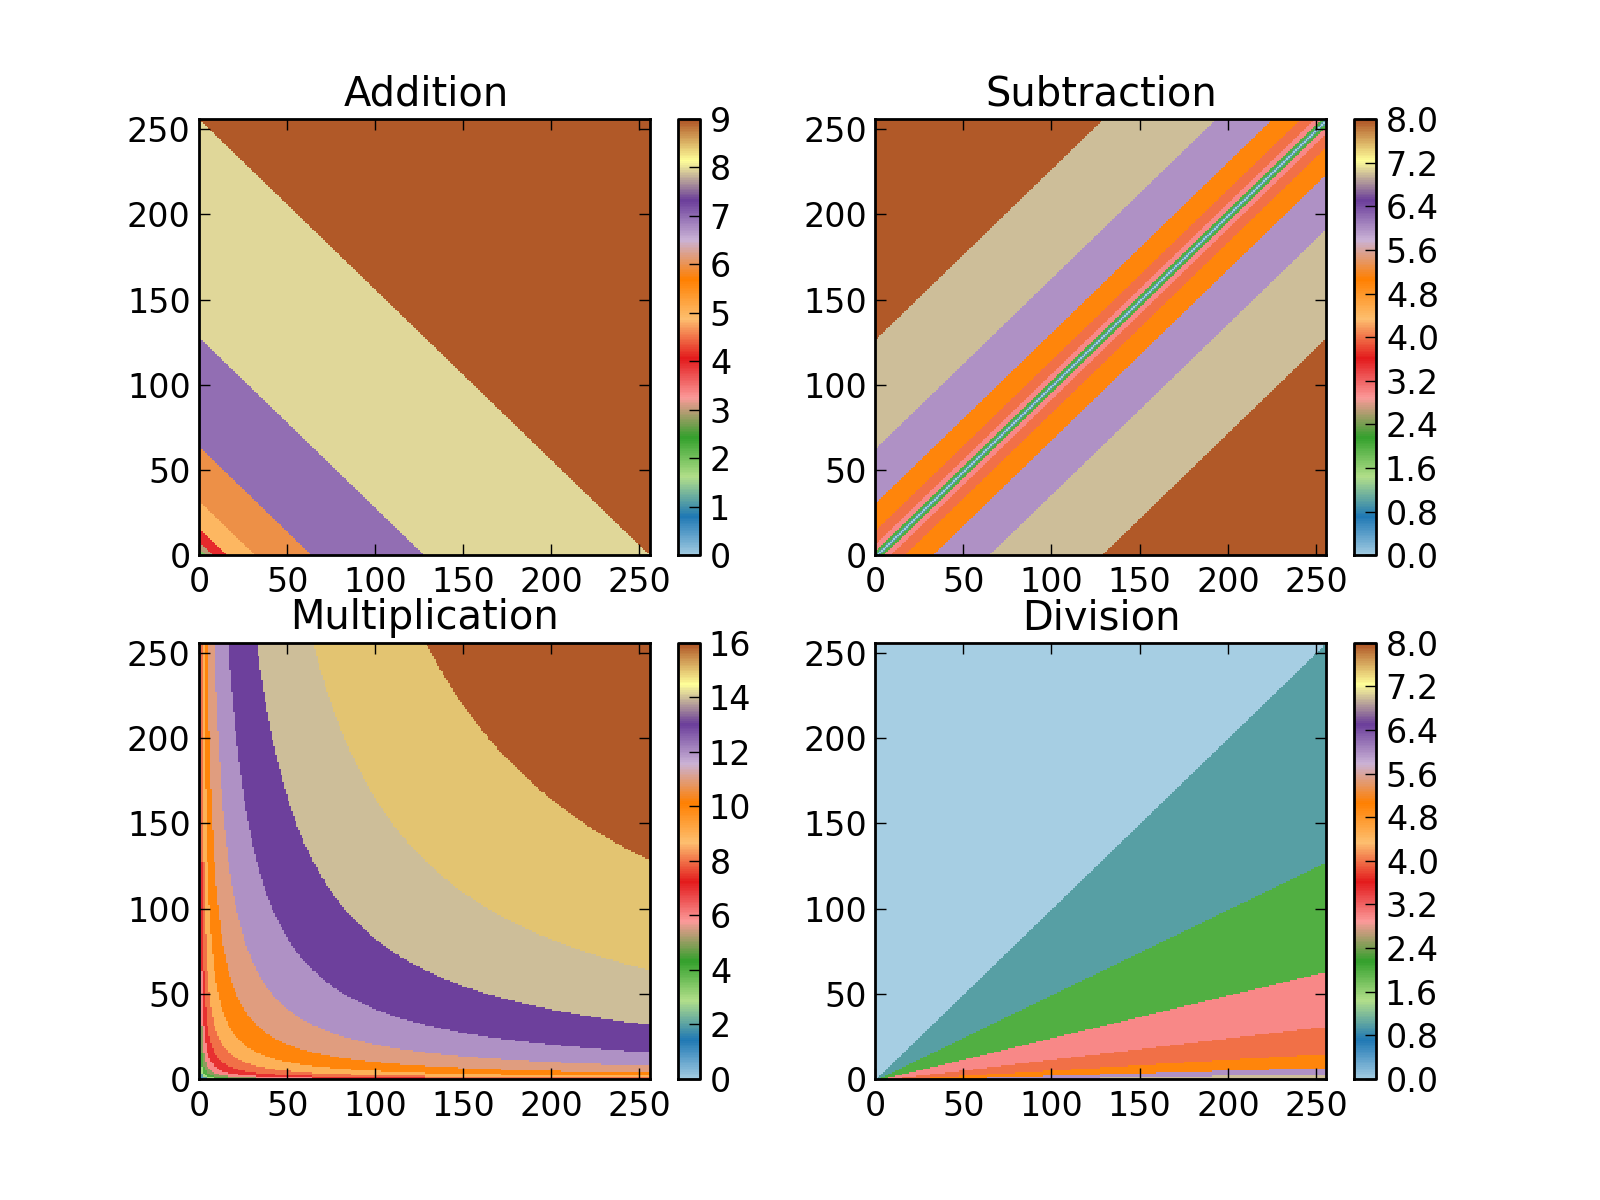
\includegraphics[width=12cm]{./bitlength.png}
 \caption{Bit-length of the results for each of the four operations. The axes
represent the values of the operands.}
 \label{fig:bitlength}
\end{figure}

\subsection{Operation on Bitstrings}

To illustrate operations with bitstrings, consider the matrices $A$ an $B$,
both $3 \times 4$:

\begin{equation}
	A = \begin{bmatrix}
			1 & 3 & 5 & 8\\ 
			12 &14  & 6 & 9\\ 
			3 & 7 & 10 & 11
		\end{bmatrix}
\end{equation}

and

\begin{equation}
	B = \begin{bmatrix}
			1  & 3  & 7 & 9\\ 
			1  &3   & 14 & 15\\ 
			20 & 30 & 2 & 1
		\end{bmatrix}
\end{equation}

After bitstring compression by the SM method, they become $3 \times 1$. They
are show in decimal and binary from in \ref{eq:01} and
\ref{eq:02}. The elements in $A$ and $B$ are 4 and 5 bits long, respectively
(the ``supreme minimum''). The ellipses (``$\ldots$'') in the binary matrix
correspond the extra zeros to the left. Since the strings are written into 64
bits integers, sometimes we end up with unused bits to the left.

\begin{equation}\label{eq:01}
	AA = \begin{bmatrix}
			4952\\ 
			52841\\ 
			14251
		\end{bmatrix} 
        =
        \begin{bmatrix}
			\ldots0001001101011000\\ 
			\ldots1100111001101001\\ 
			\ldots0011011110101011
		\end{bmatrix}
        =
        \begin{bmatrix}
\ldots\underbrace{0001}_{1}\underbrace{0011}_{3}\underbrace{0101}_{5}\underbrace
{1000}_{8}\\
\ldots\underbrace{1100}_{12}\underbrace{1110}_{14}\underbrace{0110}_{6}
\underbrace{1001}_{9}\\ 
\ldots\underbrace{0011}_{3}\underbrace{0111}_{7}\underbrace{1010}_{10}
\underbrace{1011}_{11}
	\end{bmatrix}
\end{equation}

and

\begin{equation}\label{eq:02}
	BB = \begin{bmatrix}
			36073\\ 
			36303\\ 
			686145
		\end{bmatrix}
        =
         \begin{bmatrix}
			\ldots00001000110011101001\\ 
			\ldots00001000110111001111\\ 
			\ldots10100111100001000001
		\end{bmatrix}
        =
        \begin{bmatrix}

\ldots\underbrace{00001}_{1}\underbrace{00011}_{3}\underbrace{00111}_{7}
\underbrace{01001}_{59}\\
\ldots\underbrace{00001}_{1}\underbrace{00011}_{3}\underbrace{01110}_{14}
\underbrace{01111}_{15}\\
\ldots\underbrace{10100}_{20}\underbrace{11110}_{30}\underbrace{00010}_{2}
\underbrace{00001}_{1}
		\end{bmatrix}
\end{equation}

Consider now just the bitstring stored in the first line of each matrix ($AA$
and $BB$). To recover the original elements we need to now the bit-length of
the blocks of memory containing them, for the SM method they are all the same
length. To obtain the values in an efficient way, we will use a binary mask.
The mask will recover the first and third blocks at the same time to save time.
The mask is stored as a bitstring the same length as those storing the matrix
elements. The mask for the first and third elements of matrix $AA$ is depicted
in \ref{eq:06}. To recover the second and fourth elements, we apply the mask
shown on \ref{eq:07}. For Matrix $BB$, see \ref{eq:08} and \ref{eq:09} for the
respective masks.

\begin{equation}\label{eq:06}
\text{Matrix AA's mask for positions 1 and 3} = \ldots0000111100001111
\end{equation}

\begin{equation}\label{eq:07}
\text{Matrix AA's mask for positions 2 and 4} = \ldots1111000011110000
\end{equation}

\begin{equation}\label{eq:08}
\text{Matrix BB's mask for positions 1 and 3} = \ldots00000111110000011111
\end{equation}

\begin{equation}\label{eq:09}
\text{Matrix BB's mask for positions 2 and 4} = \ldots11111000001111100000
\end{equation}

Once defined the mask we can apply it to matrices $A$ and $B$. We use the mask
by applying the boolean function AND. Let $tempA$ and $tempB$ the recovered
elements. The recovering process is illustrated below. Note that only the
positions where the mask is $1$ are retained.

  \begin{align*}
   A[1,1]		&=	\ldots0001|0011|0101|1000\\
   \text{mask A}	&=	\ldots0000|1111|0000|1111\\
   tempA 		&=	\ldots0000|0011|0000|1000
  \end{align*}

  \begin{align*}
   B[1,1]		&= \ldots00001|00011|00111|01001 \\
   \text{mask B}	&= \ldots00000|11111|00000|11111 \\
   tempB 		&= \ldots00000|00011|00000|01001
  \end{align*}

\paragraph{Addition}

Suppose we want to add both matrices and store it in a matrix $S$. for that the
blocks of $tempA$ and $tempB$ must have the same length. As for the addition we
need, in the worst case, an extra bit, the block length of the resulting
bitstring will be 6. The string from each matrix, padded on the left towards
this new length,  are shown in equations \ref{eq:12} and \ref{eq:13}.

\begin{equation}\label{eq:12}
tempA =  \ldots\textbf{00}0000\textbf{00}0011\textbf{00}0000\textbf{00}1000
\end{equation}

\begin{equation}\label{eq:13}
tempB =  \ldots\textbf{0}00000\textbf{0}00011\textbf{0}00000\textbf{0}01001
\end{equation}

Now that the blocks are matched in length we can perform the operation $S[1,1] =
tempA + tempB$. The operation is repeated for the second and fourth regions.
these operations can be done in parallel and the result, $S[1,1]$, is already
in compressed form.

\begin{align*}
 tempA&= \ldots000001|000011|000101|001000\\
 tempB&= \ldots000001|000011|000111|001001\\
 S[1,1]&=\ldots000010|000110|001100|010001
\end{align*}

We can see below the same operation performed for bitstrings $S[2,1]$ and
$S[3,1]$.

\begin{align*}
 tempA&= \ldots001100|001110|000110|001001\\
 tempB&= \ldots000001|000011|001110|001111\\
 S[2,1]&=\ldots001101|010001|010100|011000
\end{align*}

\begin{align*}
 tempA&= \ldots000011|000111|001010|001011 \\
 tempB&= \ldots010100|011110|000010|000001 \\
 S[3,1]&=\ldots010111|100101|001100|001100
\end{align*}

Therefore, as the final result of the operation $S= A + B$, we have:

\begin{align}
	S &=\begin{bmatrix}
	      549649\\ 
	      274889\\ 
	      6181644
	    \end{bmatrix}
        =
        \begin{bmatrix}
	    \ldots000010000110001100010001\\
	    \ldots000001000011000111001001\\
	    \ldots010111100101001100001100
	\end{bmatrix}
      \\ \nonumber      
      &=\begin{bmatrix}
  \ldots\underbrace{000010}_{2}\underbrace{000110}_{6}\underbrace{001100}_{12}
  \underbrace{010001}_{17}\\	
  \ldots\underbrace{001101}_{13}\underbrace{010001}_{17}\underbrace{010100}_{20}
  \underbrace{011000}_{24}\\
  \ldots\underbrace{010111}_{23}\underbrace{100101}_{37}\underbrace{001100}_{12}
  \underbrace{001100}_{12}
	\end{bmatrix}
\end{align}

\paragraph{Subtraction}
To perform the subtraction, we need to use C2 notation. Suppose  we need to
calculate $D = B - A$. This operation can be done in the same way, by
converting it to an addition: $D = B + (-A)$, where $-A$ will be converted to
C2 (equation \ref{eq:ac2}). Note the elements will be calculated with six
digits.

\begin{align}\label{eq:ac2}
	-A &= \begin{bmatrix}
		4952\\ 
		52841\\ 
		14251
	      \end{bmatrix} 
        =
        \begin{bmatrix}
	  \ldots111111111101111011111000\\ 
	  \ldots110100110010111010110111\\ 
	  \ldots111101111001110110110101
	\end{bmatrix}
        \\\nonumber
        &=\begin{bmatrix}
\ldots\underbrace{111111}_{-1}\underbrace{111101}_{-3}\underbrace{111011}_{-5}
\underbrace{111000}_{-8}\\
\ldots\underbrace{110100}_{-12}\underbrace{110010}_{-14}\underbrace{111010}_{-6}
\underbrace{110111}_{-9}\\
\ldots\underbrace{111101}_{-3}\underbrace{111001}_{-7}\underbrace{110110}_{-10}
\underbrace{110101}_{-11}
	  \end{bmatrix}
\end{align}

Now we apply the masks as before, but before we need to convert to C2 as well,
in order to perform the addition.

To exemplify, let's examine closely the operations $B[1,1] + (-A[1,1])$,
$B[2,1] + (-A[2,1])$ and $B[3,1] + (-A[3,1])$. We use $tempB$ to store each line
of the matrix B converted to C2. The numbers $1$ marked in the bitstring, are
overflows and must be removed. The result is shown below:

\begin{align*}
	tempB	&=\ldots000001|000011|000111|001001\\
    +(-A[1,1])	&=\ldots111111|111101|111011|111000\\
	D[1,1]
&=\ldots\sout{1}000000|\sout{1}000000|\sout{1}000010|\sout{1}000001
\end{align*}

\begin{align*}
	tempB 	&= \ldots000001|000011|001110|001111\\
      +(-A[2,1])&= \ldots110100|110010|111010|110111\\ 
      D[2,1]	&= \ldots110101|110101|\sout{1}001000|\sout{1}000110
\end{align*}

\begin{align*}
    tempB	&= \ldots010100|011110|000010|000001 \\
    +(-A[3,1])	&= \ldots111101|111001|110110|110101\\ 
    D[3,1]	&= \ldots\sout{1}010001|\sout{1}110111|\sout{1}111000|110110
\end{align*}

After the removal of the overflows, matrix $D$ becomes:

\begin{align}
	D &=\begin{bmatrix}
		129\\ 
		14111238\\ 
		4685366
	    \end{bmatrix} 
        =
        \begin{bmatrix}
	  \ldots000000000000000010000001 \\
	  \ldots110101110101001000000110 \\
	  \ldots010001110111111000110110
	\end{bmatrix}
	\\\nonumber
	&=\begin{bmatrix}
\ldots\underbrace{000000}_{0}\underbrace{000000}_{0}\underbrace{000010}_{2}
\underbrace{000001}_{1} \\ 			 
\ldots\underbrace{110101}_{-11}\underbrace{110101}_{-11}\underbrace{001000}_{8}
\underbrace{000110}_{6} \\
\ldots\underbrace{010001}_{17}\underbrace{110111}_{23}\underbrace{111000}_{-8}
\underbrace{110110}_{-10}
	  \end{bmatrix}
\end{align}

\paragraph{Multiplication}

Let's now examine matrix multiplication. Consider the product $P = A \times
B^{t}$, where $B^t$ is the transpose of B. Thus the product becomes:

\begin{equation}
	P = A \times B = \begin{bmatrix}
		1 & 3 & 5 & 8\\ 
		12 &14  & 6 & 9\\ 
		3 & 7 & 10 & 11
		\end{bmatrix}
        \times
		\begin{bmatrix}
		  1 & 1  & 20\\ 
		  3 & 3  & 30\\
		  7 & 14 & 2\\
		  9 & 15 & 1
		\end{bmatrix}
\end{equation}

Again, using $AA$ and $BB$ to denote the compressed versions of the matrices,
and $\times\times$ to denote the multiplication of bitstring matrices, the
compressed product becomes:

\begin{equation}\label{eq:prodbs}
	P = AA \times BB =\begin{bmatrix}
			    4952\\ 
			    52841\\ 
			    14251
			  \end{bmatrix} 
        \times\times
	\begin{bmatrix}
	  36073 & 36303 & 686145
	\end{bmatrix}
\end{equation}

\begin{equation}
	P = AA \times BB = 
    	\begin{bmatrix}
\ldots\underbrace{0001}_{1}\underbrace{0011}_{3}\underbrace{0101}_{5}\underbrace
{1000}_{8}\\
\ldots\underbrace{1100}_{12}\underbrace{1110}_{14}\underbrace{0110}_{6}
\underbrace{1001}_{9}\\
\ldots\underbrace{0011}_{3}\underbrace{0111}_{7}\underbrace{1010}_{10}
\underbrace{1011}_{11}
	\end{bmatrix}
\end{equation}

\begin{small}
  \begin{equation}
	  \times\times \\
	  \begin{bmatrix}\mathsf{
\ldots\underbrace{00001}_{1}\underbrace{00011}_{3}\underbrace{00111}_{7}
\underbrace{01001}_{9}}  &\mathsf{
\ldots\underbrace{00001}_{1}\underbrace{00011}_{3}\underbrace{01110}_{14}
\underbrace{01111}_{15}} & \mathsf{
\ldots\underbrace{10100}_{20}\underbrace{11110}_{30}\underbrace{00010}_{2}
\underbrace{00001}_{1}}
	  \end{bmatrix}\nonumber
  \end{equation}
\end{small}

To calculate $P[1,1]$ which in uncompressed form is $1 \times 1 + 3 \times 3 + 5
\times 7 + 8 \times 9$, we first must extract the numbers from the bitstrings
and then proceed with the linear combination. The extraction will make use of
masks as described before. Let $tempA$ and $tempB$ store the values of blocks 1 
and 3 of AA[1,1] and BB[1,1]. Now we need to determine the size of the blocks
(bit-length) containing each element of the resulting matrix. As demonstrated
before, in the worst case, the product will have a bit-length which is the sum
of the bit-lengths of the operands. For this example this length is $4+5=9$,
however, we also have three additions for each element,adding a total of 3
extra bits, thus we end up with a bit-length of 12 for each element of the
product. Having determined the bit-length of the product, we can now do the 
actual calculations and store the results.

The linear combination of elements which generates $P[1,1]$ is detailed below.
We use temporary variables $tempP_i$ to store the products before adding them,
where $i$ is the product being calculated.

\begin{align*}
 tempA&= \ldots0001|0011|0101|1000\\
 tempB&= \ldots00001|00011|00111|01001\\
\end{align*}

\begin{align*}
 tempA&= \ldots\textbf{0001}|0011|0101|1000\\
 tempB&= \ldots\textbf{00001}|00011|00111|01001\\
 tempP_1&= \ldots000000001
\end{align*}

\begin{align*}
 tempA&= \ldots0001|\textbf{0011}|0101|1000\\
 tempB&= \ldots00001|\textbf{00011}|00111|01001\\
 tempP_2&= \ldots000001001
\end{align*}

\begin{align*}
 tempA&= \ldots0001|0011|\textbf{0101}|1000\\
 tempB&= \ldots00001|00011|\textbf{00111}|01001\\
 tempP_3&= \ldots000100011
\end{align*}

\begin{align*}
 tempA&= \ldots0001|0011|0101|\textbf{1000}\\
 tempB&= \ldots00001|00011|00111|\textbf{01001}\\
 tempP_4&= \ldots001001000
\end{align*}

\begin{align*}
 tempP1&= \ldots0000000001 \\
 tempP2&= \ldots0000001001 \\
   soma&= \ldots0000001010 \text{ (10 bits)}
\end{align*}

\begin{align*}
 tempP3&= \ldots00000100011 \\
   soma&= \ldots00000001010 \\
   soma&= \ldots00000101101 \text{ (11 bits)}
\end{align*}

\begin{align*}
 tempP4&= \ldots000001001000 \\
 soma&=   \ldots000000101101 \\
 soma&=   \ldots000001110101 \text{ (12 bits)}
\end{align*}

So, $P[1,1]$ is $000001010101$, and the entire matrix $P$ becomes:

\begin{align}
	P &= \begin{bmatrix}
			1426882688\\ 
			2970686121\\ 
			3239350573
		\end{bmatrix} 
        =
        \begin{bmatrix}
   			\ldots000001010101000011001000000010000000 \\
			\ldots000010110001000100010001001010101001\\
			\ldots000011000001000101001001000100101101
		\end{bmatrix}
      \\ \nonumber
        &=        \begin{bmatrix}
\ldots\underbrace{000001010101}_{117}\underbrace{000011001000}_{200}\underbrace{
000010000000}_{128}\\
\ldots\underbrace{000010110001}_{177}\underbrace{000100010001}_{273}\underbrace{
001010101001}_{681}\\
\ldots\underbrace{000011000001}_{193}\underbrace{000101001001}_{329}\underbrace{
000100101101}_{301} 			 
        \end{bmatrix}
\end{align}

Again, we can see that P is already in compressed form, which confirms that the
entire operation was conducted without decompressing the data.

The division operation with matrices will be described in a subsequent paper
after we describe how to represent and operate with floating-point numbers.

In the examples given above, we only used the SM method, but the same procedure
can be easily adapted to the VLB method.

Thus we complete our demonstration of how to perform basic arithmetic
operations with bitstring compressed scalars and matrices.

\section{Implementation}

This paper proposes the bitstring-compression methodologies. The SM 
method was implemented as a Fortran library which is available under an 
open-source license. The 
implementation extends the standard Matrix type of Fortran, overloading 
operators such as assignment, addition, subtraction, multiplication, transpose, 
and maximum of a matrix. 
Although only few significant matrix operations have been ovearloaded in this 
example implementation, any other operation can be performed, since 
the methods for inserting and collecting an element in a matrix of bitstring 
were also implemented. With these two methods, as long as they are properly 
adapted into algorithms, it is possible to implement any other desired 
operation.

The SM method was also extended to allow for the allocation of real and 
signed integer matrices, besides positive integer ones. Some adjustments were 
made so that the other types of numbers could be represented. \todo{removi 
``in order to represent...''}

The SM method uses a fixed number of bits to store the values in such a way that
the size or number of bits used is important to represent the highest value in 
the bitstring matrix. The adaptation 
consists in determining the largest value to be stored considering the absolute 
value of the number. That done,
when the number is negative, it is necessary to rewrite it since, due to the 
sign, this will be written in the form of 
two's complement. The purpose of this conversion is to optimize library 
processing. Take the following as an example: 
the number 5, when represented in a 32-bit integer, is defined as:

\begin{equation}\nonumber
 5 = 00000000 00000000 00000000 00000101
\end{equation}

However, if the number is negative, this is represented in the form of two's 
complement. Therefore, the number -5 is 
represented as:

\begin{equation}\nonumber
 -5 = 11111111 11111111 11111111 11111011
\end{equation}

Note that the bit positioned more to the left should be used to inform that the 
number is -5. For the purpose of 
optimization of the library, it was chosen to conversion of positive numbers to 
negative numbers and use of 1 
bit to represent the sign. (Dúvidas aqui)

In turn, in order to represent real numbers, a conversion procedure of real 
numbers to integer numbers was used. The 
real number is multiplied by a power of ten and is then immediately truncated. 
The real numbers in a binary system of 64 
bits are represented using a bit to represent the sign of the number, 11 bits to 
the exponent, and 52 bits to the 
mantissa. Note that 1 bit is still used implicitly, according to the IEEE-754 
standard. In summary, the mantissa is 
represented in the base $2^{-1}$, $2^{-2}$, $2^{-3}$, $\hdots$, $2^{-52}$. 
Depending on the value to be represented, 
loss of information can take place, which is related to the accuracy of the type 
used. In this case, considering a real 
number with double precision, the demand of 64 bits to represent each one 
occurs, and in some cases, the number to be 
represented is an approximation. As an example, consider that the number to be 
stored is 1.109. Following the 
traditional system, the number 1,109 is represented by

\begin{equation}\nonumber
  0011111111110001101111100111011011001000101101000011100101011000
\end{equation}

We consider that the power used is $10^3$, that is, the number which needs to be 
stored would be 1109. In binary, that 
number is represented by 10001010101. Note that the number of bits required is 
smaller, but depending on numerical 
accuracy, the compression methods suggested are ineffective. When the power of 
10 is used, it must be applied across the 
matrix. This conversion allows the proposed methods to be applied to a set of 
real numbers. It should be taken into 
account that the greater the power of 10 used, which is associated with the 
conversion of the real number, the larger 
the set of bits will be required to represent the converted number. This affects 
the efficiency of data compression. The 
use of the library to represent real numbers is conditioned to a study of the 
necessary level of precision to solve the 
problem.

\section*{Library Application}

In order to create an application, some elementary matrix operations. Different 
operations have been performed by 
measuring the execution time of each. We basically, considered the attribution 
of a constant to all the elements of a 
matrix; the addition, subtraction and multiplication of the elements of a matrix 
by a constant, the addition, 
subtraction and multiplication of matrices. In addition to that, the calculation 
of  the transposed matrix and the 
maximum an array were also considered. This measure was used to evaluate the 
efficiency of the method implemented when 
compared to traditional methods.

One of the characteristics of bitstring matrices is that the operations per 
column, in the case of implementation in 
Fortran, can be parallelized. This reduces the execution time, compared to 
traditional methods. Therefore, in order to 
achieve this optimization, threads implementations were used for the implemented 
operations.

As a test methodology, all the described operations were also compared to 
traditional methods. The matrix dimensions n x 
n used were $n = 10$, $100$, $1,000$, $10,000$, $20,000$ to $100,000$, by 
$10,000$. We emphasize that the matrix,  
created with a 1,000 dimension has $10^6$ elements, while the one with a 100,000 
dimension has $1 \times 10^{10}$ 
elements. With the increase of the size of the matrices, a larger amount of 
memory must be reserved to allocate the 
numbers. The compression effect of the matrices can be verified in the results 
since by the proposed method the matrix 
is ​​directly loaded into the main memory, avoiding the need for access to the 
secondary memory.

In Figures \ref{fig:23242526} and \ref{fig:27282930} the results from the 
processing time (in milliseconds) 
for the operations that involved only integer ($Z$) and positive integer numbers 
($Z^+$) are represented. 
The traditional method (Normal) and the Bitstring method (Bitstring $Z$, integer 
numbers and Bitstring Zp, 
positive integer numbers) were used. The operations were attribution ($A=5$, A 
is a matrix with dimension n by n); 
sum of the elements of a matrix with a constant ($A=A+5$); sum of matrices 
($A=A+A$); andsubtraction of the elements 
of a matrix with a constant ($A=A-8$). These operations are represented in 
Figure \ref{fig:23242526}. 
Figure \ref{fig:27282930}, in turn, shows the results for the 
multiplicationoperations of matrices ($A = A \times A$); 
for the multiplication of the the elements of a matrix by a constant ($A=A 
\times 2$); 
and for the calculation of transpose and maximum of a matrix.

The results show that the bitstring method is faster than the traditional ones 
only for the attribution.
This occurs because the element of the matrix is used more than once to store 
the numbers, differently 
from the traditional method. Due to the number of manipulations  the bitstring 
method does, the other 
operations  demand more time to be processed, but this can be optimized. When 
applied to positive integers, 
the bitstring model works faster than when applied to integers because it does 
not need to do operations 
related to the signals.

The results for the real numbers are represented in Figures \ref{fig:31323334} 
and \ref{fig:35363738}. 
By repeating the operations tested in the integer numbers, it was possible to 
see that the bitstring method 
cannot overcome the traditional method. This happensbecause its application to  
the real numbers, as alternative 
to maintain the compression, asks for a conversion of real to integer numbers in 
order for them to be stored and 
when accessed, another conversion is made. This is a problem from the 
implementation process, but it can be optimized.

Another library application was the implementation of the algorithm in order to 
deal with the problem of arrays of 
collaborative filtering \cite{cf}. These arrays have large dimensions due to the 
number of users and products. Each 
element of this matrix stores the rating of a user with respect to a specific 
product. With this information, it is 
possible to specify a product for a determined customer.

The manipulation of these matrices, depending on the amount of memory to be 
allocated, are one of the possible 
applications of the methods proposed in this work, since it promotes the 
compression and data allocation in the main 
memory. The allocation of the matrix within the main memory makes the access 
time to the elements much smaller than when 
the matrix is stored in secondary memory. This latter type of storage is used in 
some already mentioned techniques. As 
an example, let us examine the manipulation of a CF matrix, evaluating the 
access time to the elements and especially 
the size of the memory required to run such operation. The algorithms applied to 
this matrix were the average per-use 
and the bias from mean \cite{cf}, this last one of the simplest algorithms for 
predicting the rate of users.

An example of the application of the methodology presented is shown in Figure 
\ref{fig22}. In this figure, the matrix 
with normal and bitstring formats are displayed. In both matrices, the 
information is represented and can be accessed. 
Therefore, it becomes possible to apply the selected algorithms.

In order to test a possible model application, we considered a matrix with the 
following dimensions: 95,000 users 
(lines) by 3,000 movies (columns), with the ratings for Netflix’s movies
\footnote{http://graphlab.org/downloads/datasets/}. In order to evaluate a 
larger dataset, we modified the 
NetFlix data so we could increase the dimension of the matrix to be analyzed. 
The 95,000 users correspond to 
thelines of the matrix. In orderto gradually increase the number of lines, we 
performed consecutive re-samplings 
and added them to the original matrix . As a results, we obtained a  matrix with 
600,000 lines and 3,000 columns. 
The operations used with the matrix were the Per User Average (PUA) and the 
rating estimation of a movie i using 
the Bias From Mean (BFM) \cite{cf}. The analyses were  made, considering the 
created matrix with different dimensions, 
with n from 40,000 to 600,000 by 20,000. It is important to emphasize that the 
number of columns is constant and 
equal to 3,000. The implementations of this problem were made in Fortran and 
both the developedlibrary based in 
the method SM and in the traditional form were used. Codes were inserted in the 
library in order to optimize the 
multicore processing using threads. No additional configuration was necessary to 
use the multicore processing. 
since the library detects the characteristics of the processor uses them in the 
simulations. In turn, for the 
traditional implementation, weused the optimization process and parallelization, 
which are made available by 
the processor,as the vectorization and multicore parallelization.

The results are represented in Figures \ref{fig39}, \ref{fig40} and \ref{fig41} 
for the PUA Method and in Figures 
\ref{fig42}, \ref{fig43} and \ref{fig44} for the 
BFM Methods.  A computer with 8 GB of RAM Memory, 16 GB of swap, processor core 
i7 model 870
and operational 
system Linux Debian 7.0 was used to perform this simulation. In Figure 
\ref{fig39}, it is possible to verify the approximate 
moment  when the  the storage in disk (swaap) begins to be used. This is 
indicated by the vertical green line. 
At this moment, the bitstring method becomes faster than the traditional method 
because it does not require disk 
storage due tocompressed memory representation. Note that, in the Figure 
\ref{fig40}, the traditional method is faster 
than the bitstring one before the beginning of the disk access. However, after 
it becomes necessary use the disk 
so that the matrix can be accessed and stored, , the traditional method  becames 
slower (Figura \ref{fig41}). 
These results 
indicate that the bistring method can promote the optimization of the memory use 
because the access to the main 
memories (RAM and cache) are faster than the access to secondary memories 
(disk). In Figures \ref{fig42}, 
\ref{fig43} and \ref{fig44} the 
results of the processing time for  the BFM method are represented. Once again, 
a vertical green line indicates 
the approximate moment when the disk access begins. There is a difference in 
relation to the PUA method since the 
BMF method uses the PUA values to perform its calculation. Therefore, the BMF 
method demands more memory to be 
processed, which reduces the matrix dimensions involved in the process, 
represented in the main memory. As 
indicated in Figure \ref{fig41}, for the PUA method, and Figure \ref{fig44}, for 
the BMF method, it is possible 
to verify that 
before the access to the disk, the traditional method is faster than the 
bitstring one, but once the access 
is initiated,  the bitstring method becames faster.

In spite of the simplicity of the application, it is relevant since  it allows 
for large-sized matrices to be 
allocated in memory and manipulated.

\newpage

\section*{Figure Legends}

\begin{figure}[h]
  \centering
  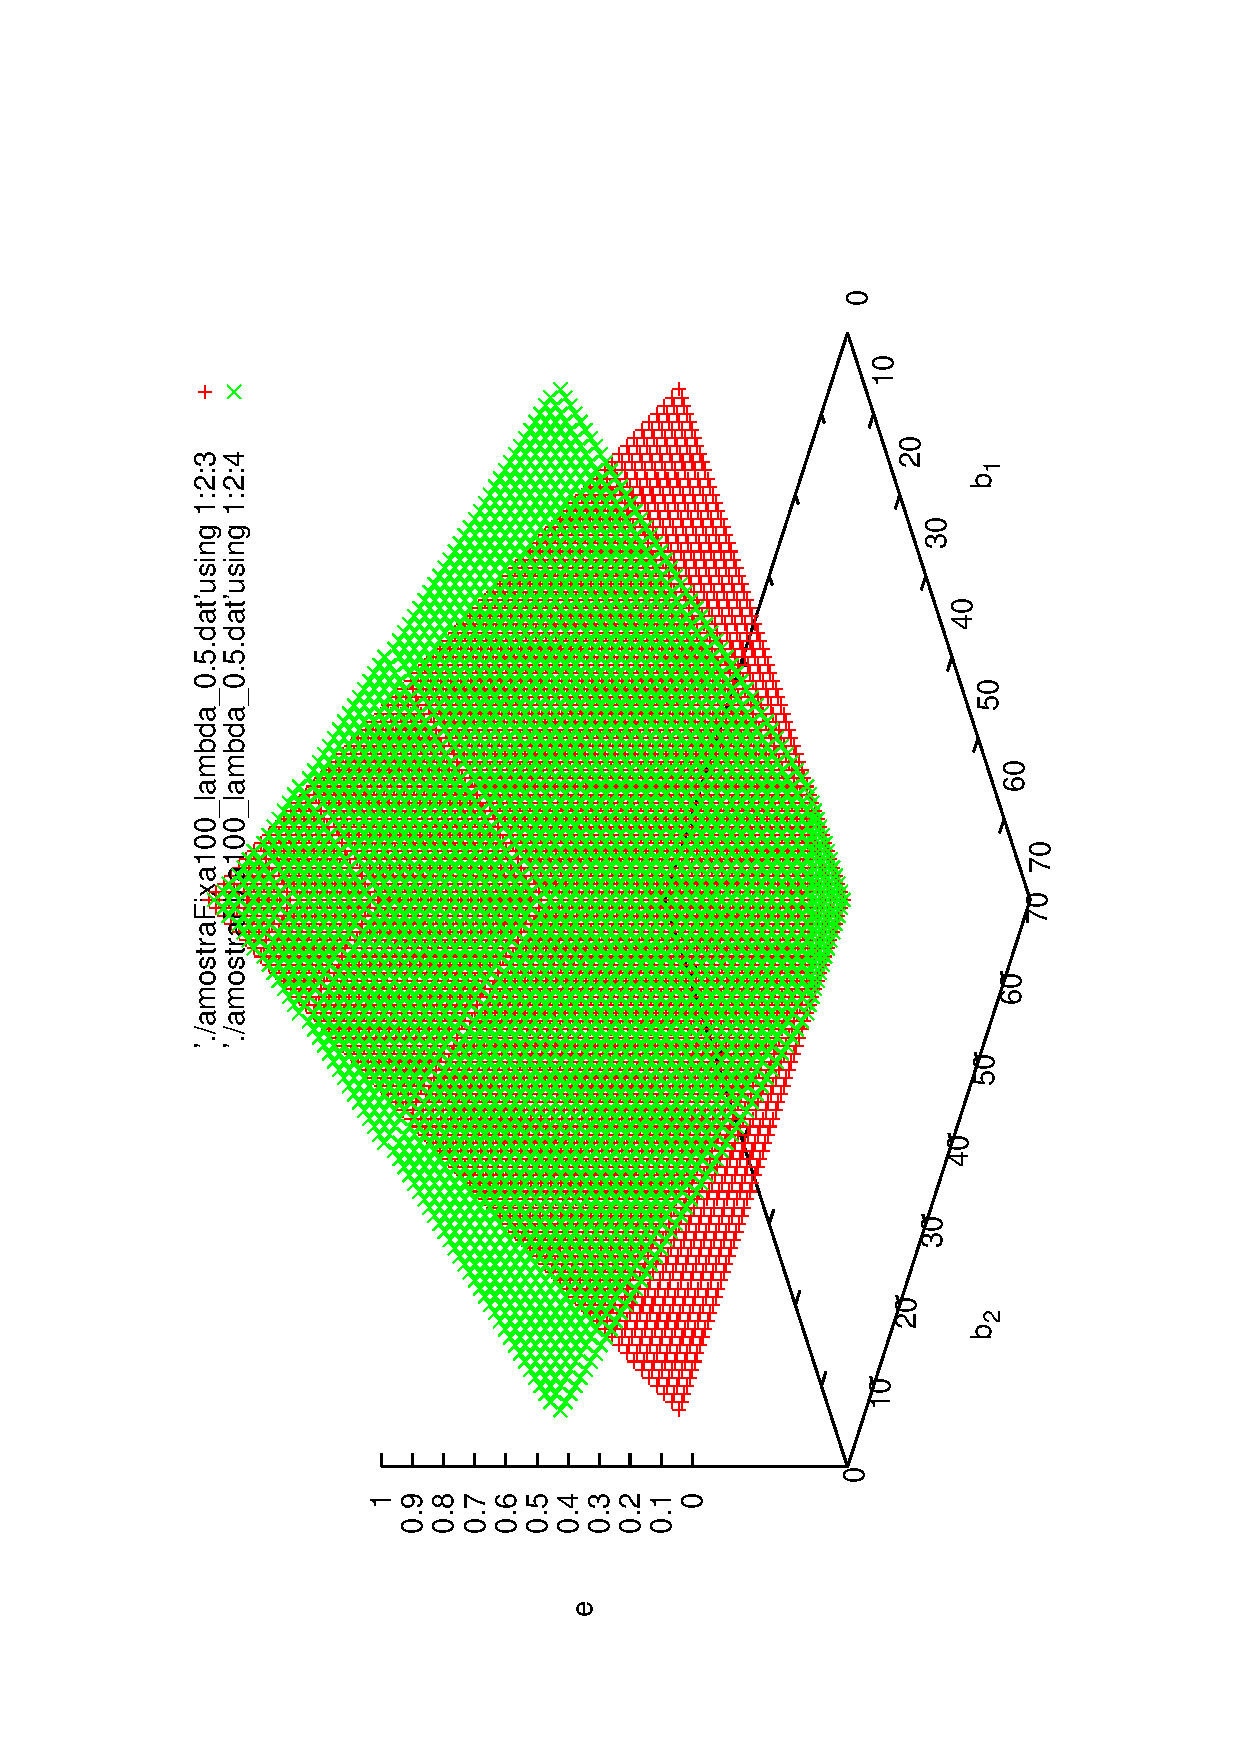
\includegraphics[scale=0.4,trim=5cm 0cm 5cm 0cm,clip]{fig22}
  \caption{Illustration of the process of the bistring model application to 
matrices of collaborative filttering of the 
algorithms per use average (PUA) and of the bias from mean (BFM) in a matrix 
represented in the traditional and 
bitstring formats.}
  \label{fig22}
\end{figure}

\begin{figure}[h]
  \centering
  \subfigure[$A=5$]{
  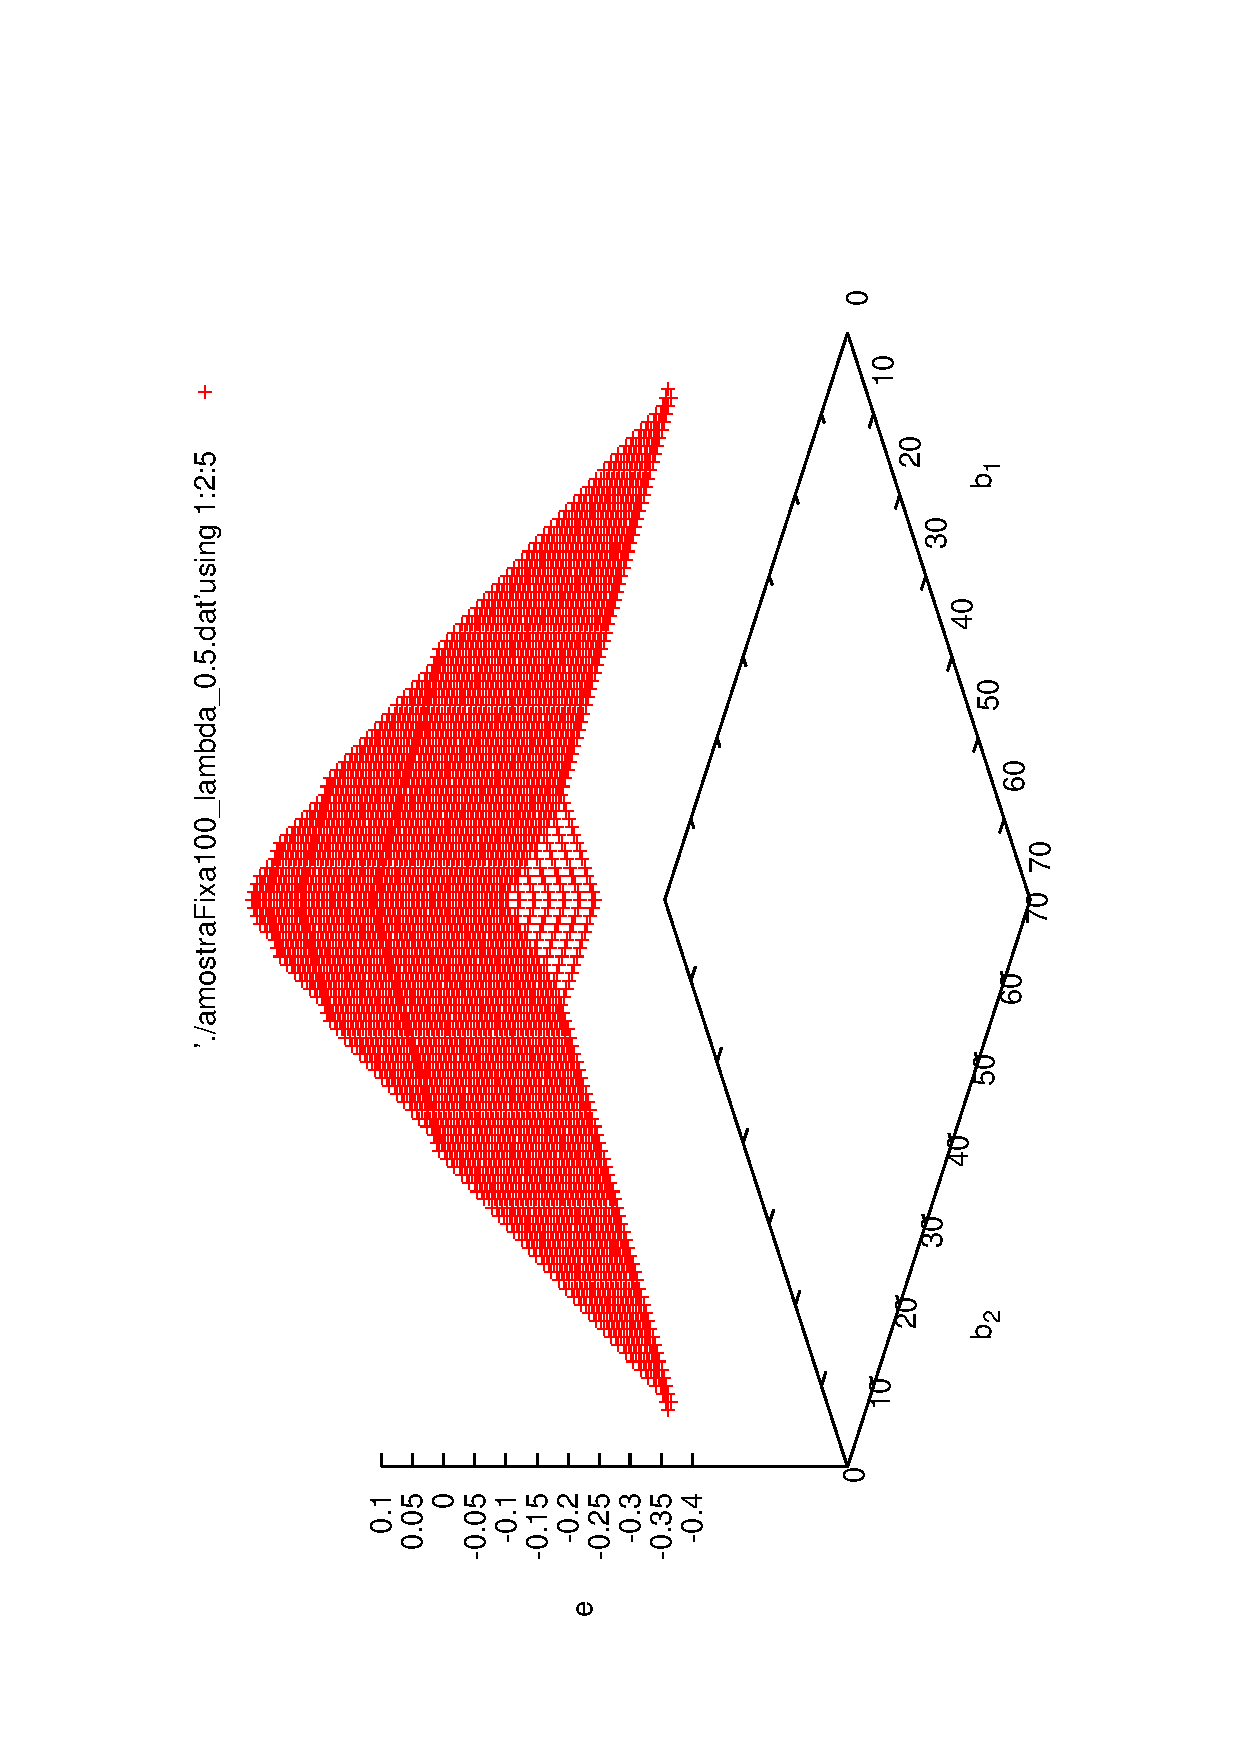
\includegraphics[scale=0.4,clip]{fig23}
  }
  \subfigure[$A=A+5$]{
  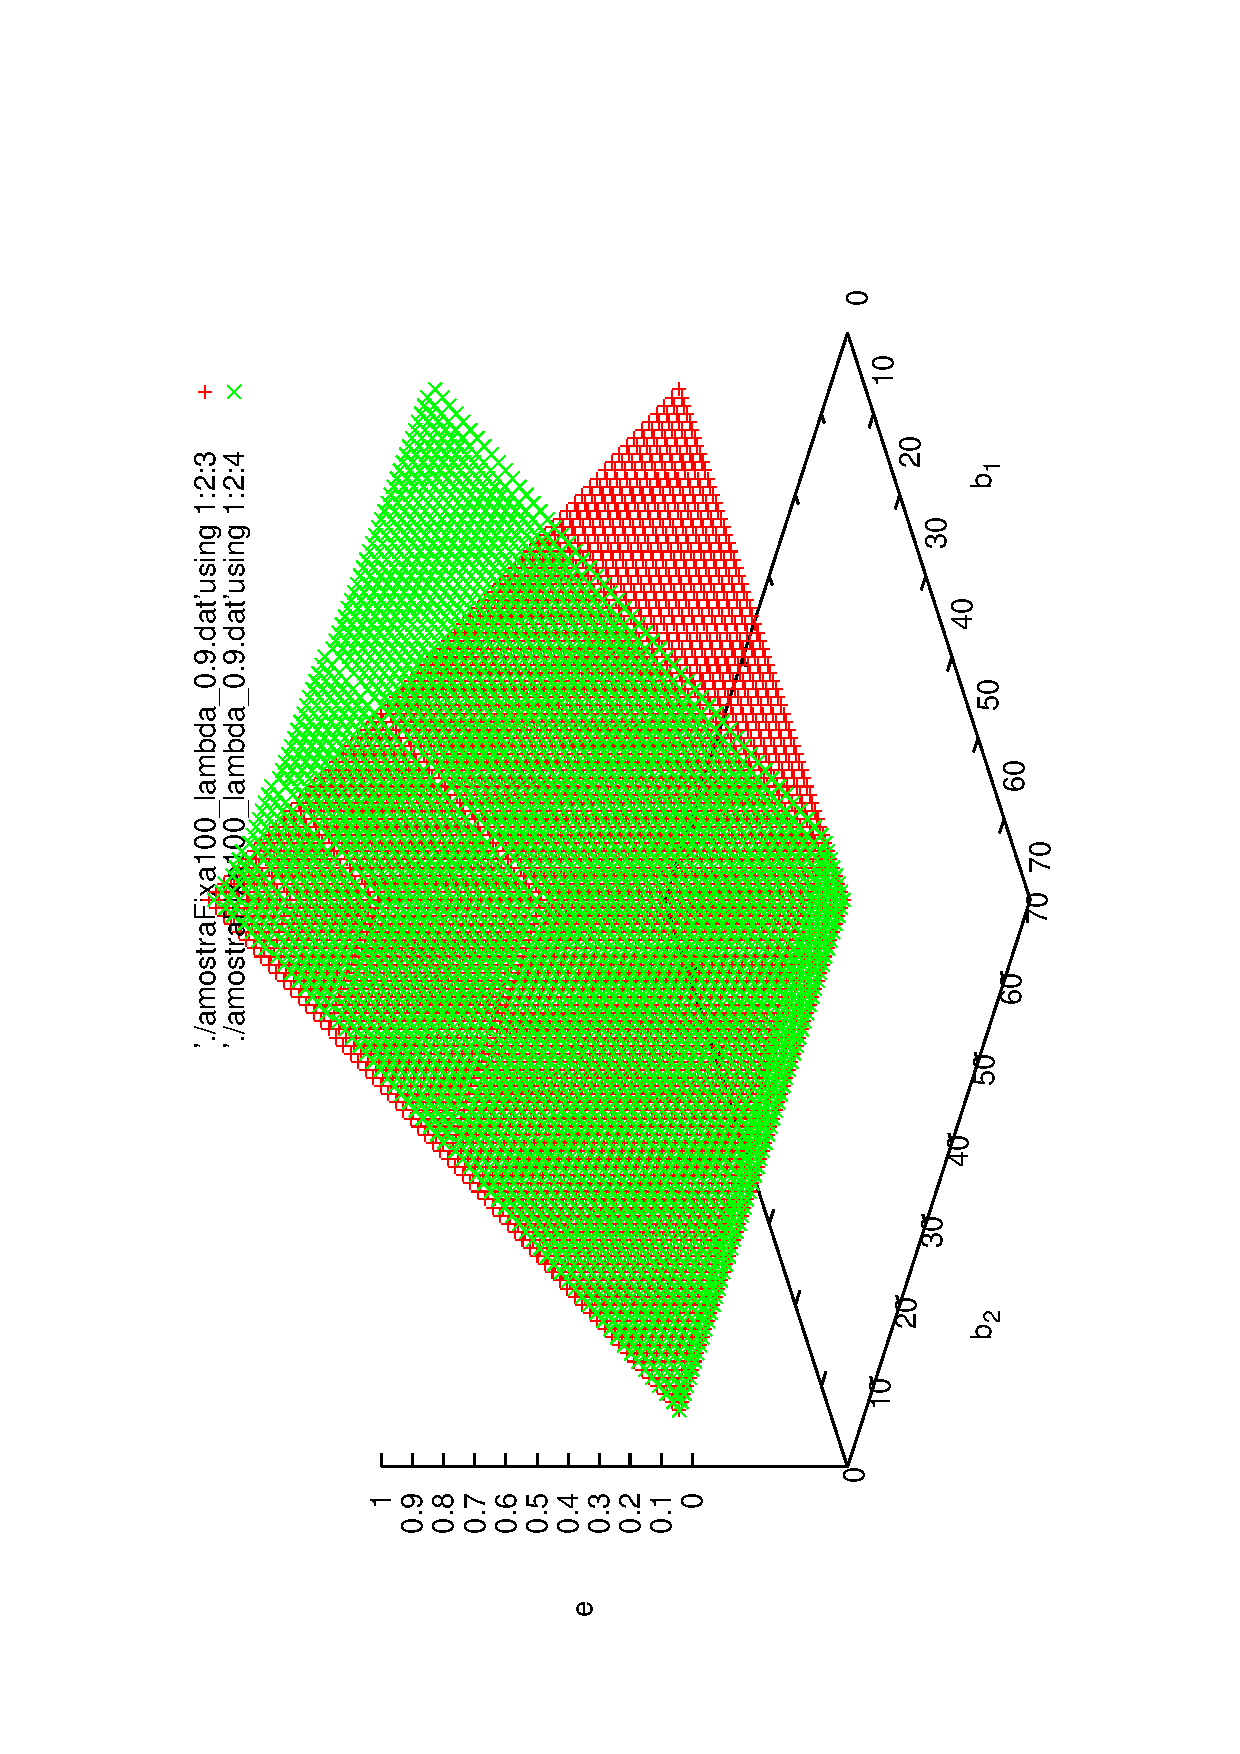
\includegraphics[scale=0.4,clip]{fig24}
  }
  \subfigure[$A=A+A$]{
  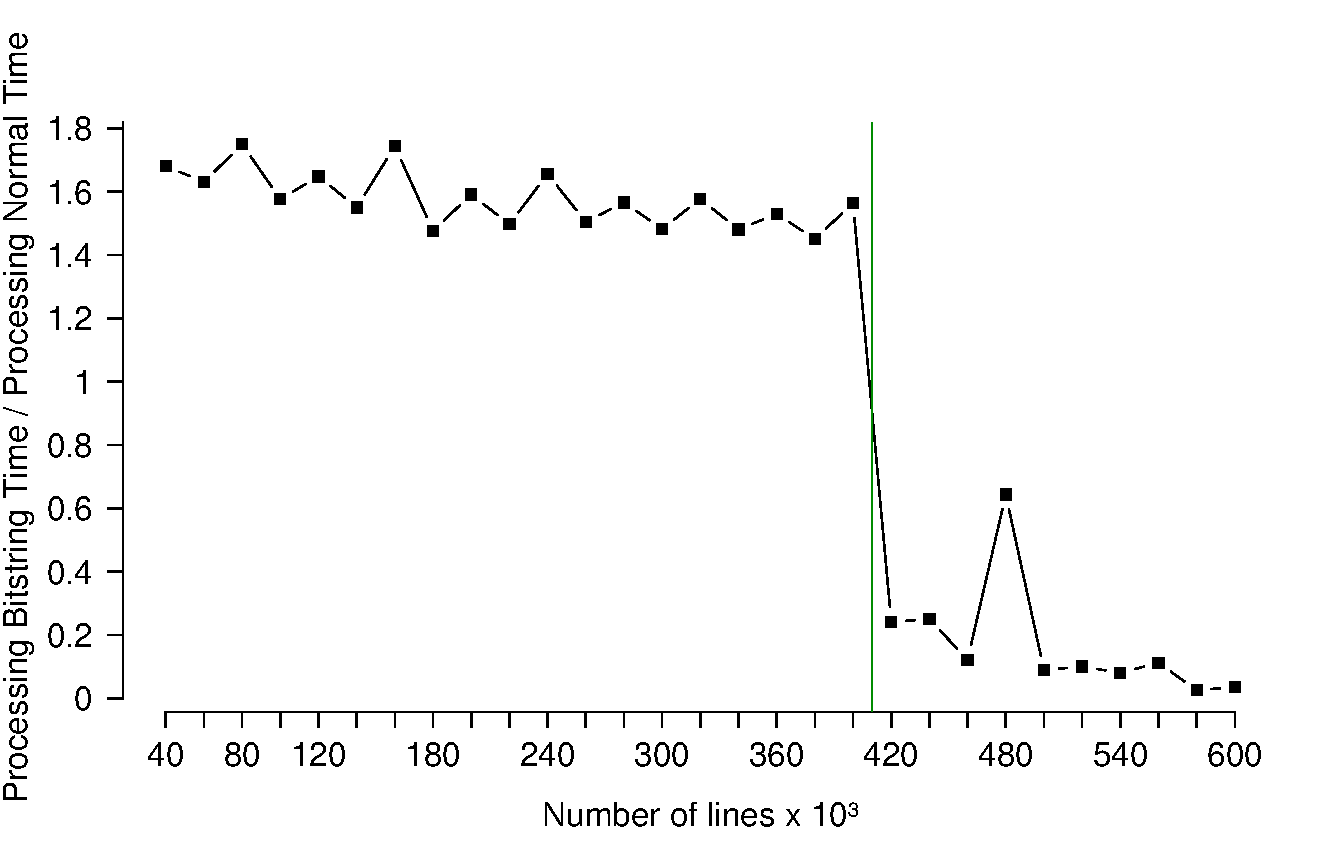
\includegraphics[scale=0.4,clip]{fig25}
  }
  \subfigure[$A=A-8$]{
  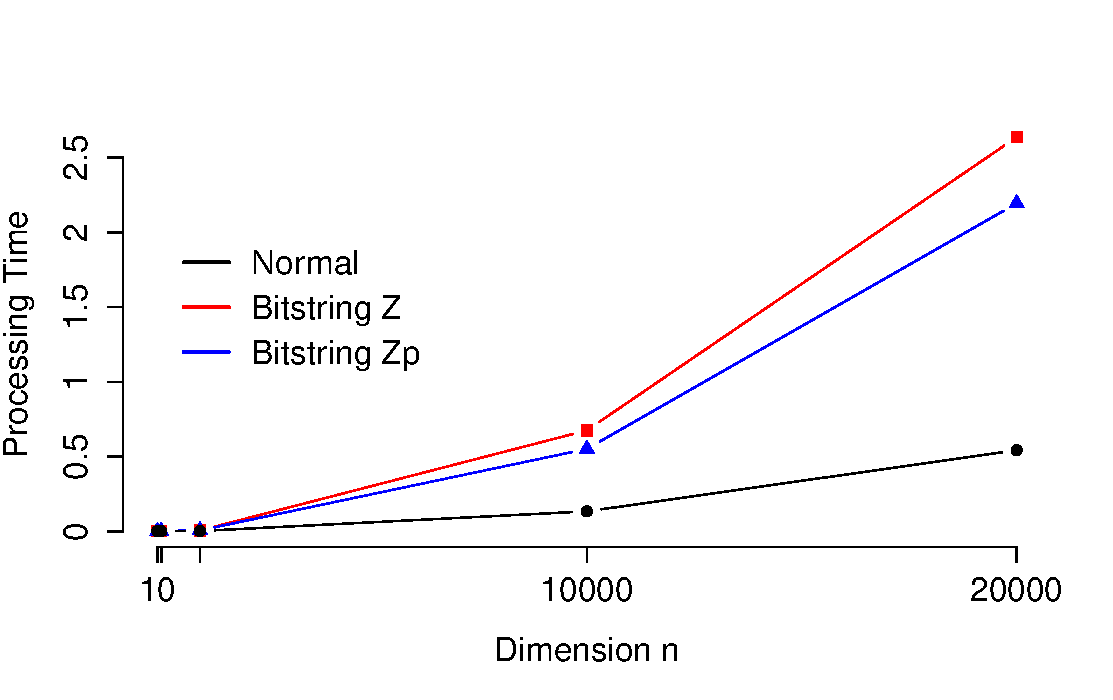
\includegraphics[scale=0.4,clip]{fig26}
  }
  \caption{Processing time of the following operations: attribution ($A=5$, A is 
the matrix with an n by n dimension); 
  element sum of a matrix with a constant ($A=A+5$);sum of matrices ($A=A+A$); 
and subtraction of the elements of a 
  matrix by a constant ($A=A-8$) involving integer numbers ($Z$) and positive 
integer numbers ($Z^+$). The bitstring 
  method presented the best overall performance only for the attribution 
operations, because the storage of 
  different numbers occurs in one element of a matrix, which reduces the 
accessing time. For the other operations, 
  the bitstring method is slower due to the number ofoperations which are 
necessary to be  executed in order to 
  access the elements. This can still be optimized in the implemented library.}
  \label{fig:23242526}
\end{figure}

\begin{figure}[h]
  \centering
  \subfigure[$A = A \times A$]{
  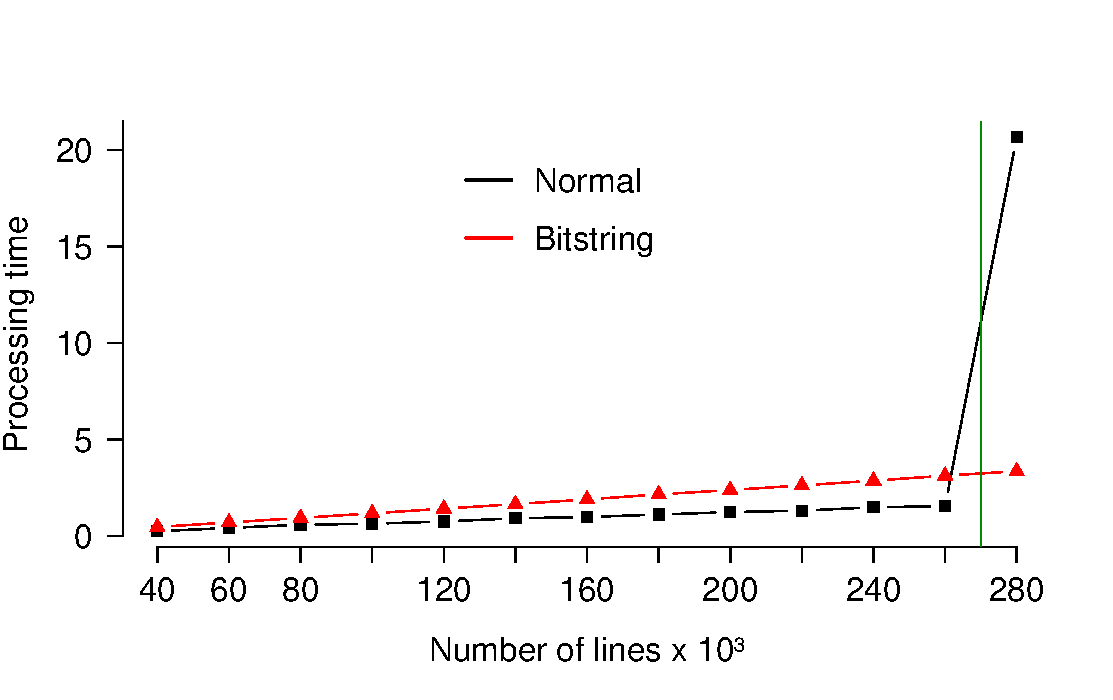
\includegraphics[scale=0.4,clip]{fig27}
  }
  \subfigure[$A=A \times 2$]{
  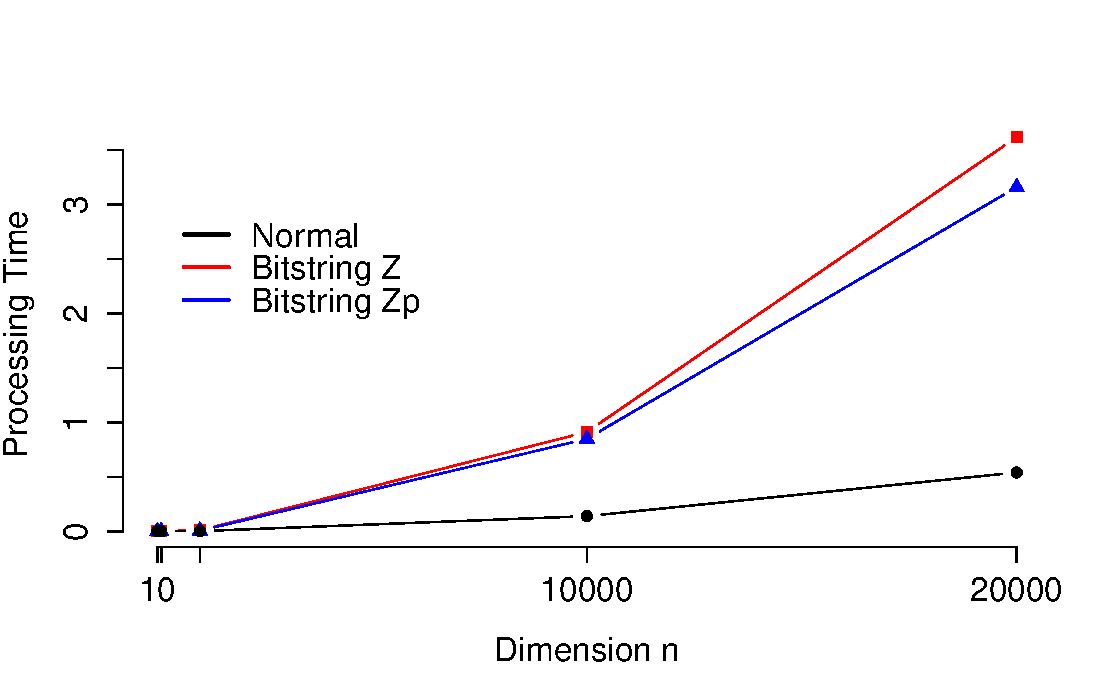
\includegraphics[scale=0.4,clip]{fig28}
  }
  \subfigure[$transpose(A)$]{
  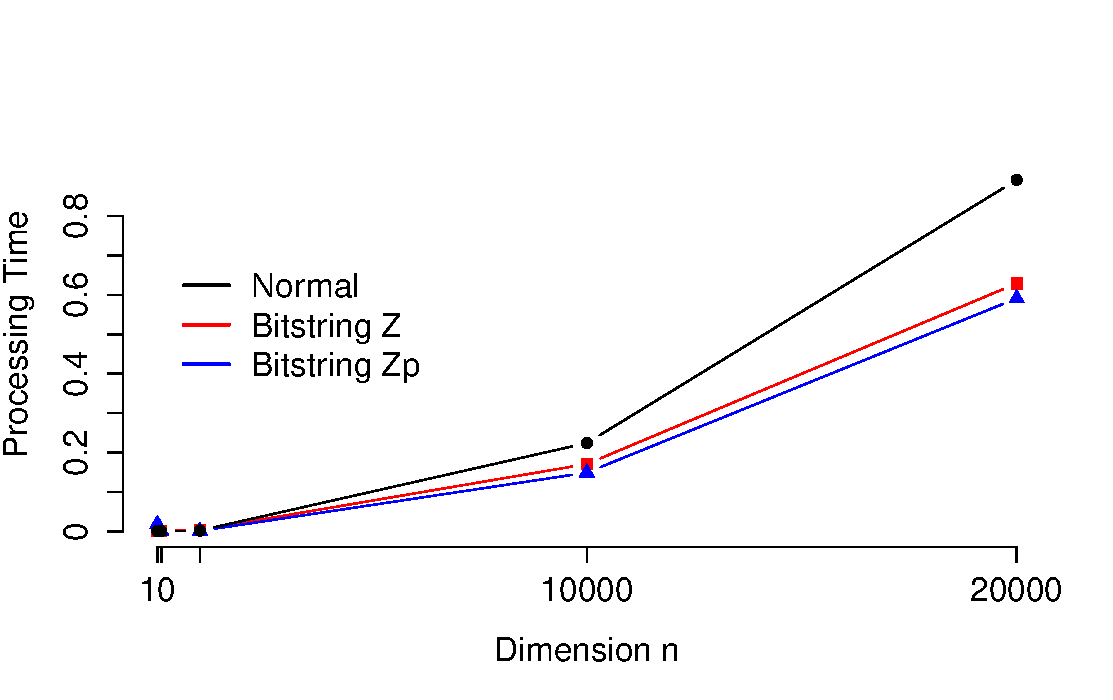
\includegraphics[scale=0.4,clip]{fig29}
  }
  \subfigure[$maximum(A)$]{
  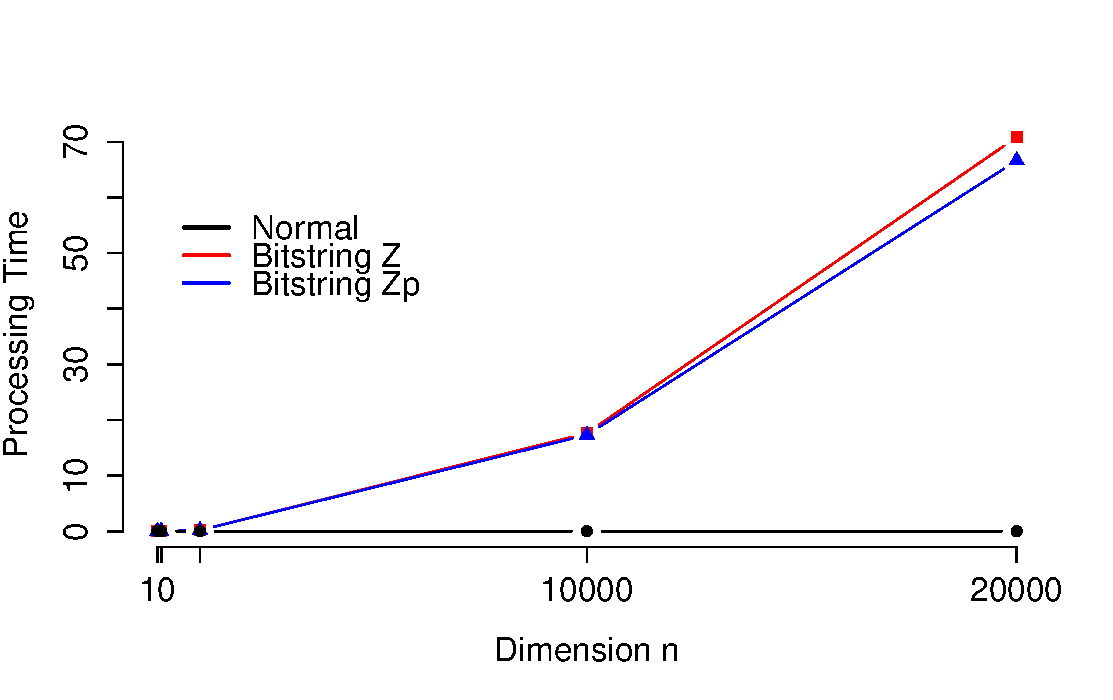
\includegraphics[scale=0.4,clip]{fig30}
  }
  \caption{Processing time of matrix multiplication ($A = A \times A$, A is the 
matrix with a n by n dimension), 
  element multiplication of matrix by constant ($A=A \times 2$), the calculation 
of transpose and maximum of a 
  matrix involve integer numbers ($Z$) and positive integer numbers ($Z^+$). In 
this cases, the traditional 
  method was faster than the bitstring model.}
  \label{fig:27282930}
\end{figure}

\begin{figure}[h]
  \centering
  \subfigure[$A=5.0000$]{
   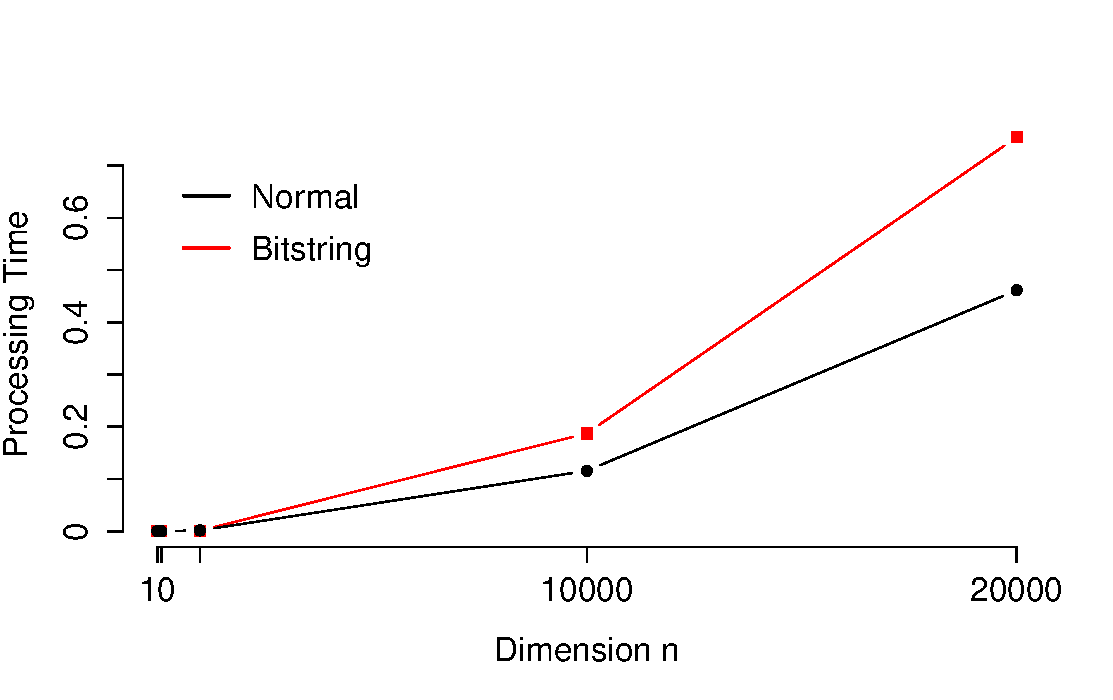
\includegraphics[scale=0.4,clip]{fig31}
  }
  \subfigure[$A=A+5.0000$]{
   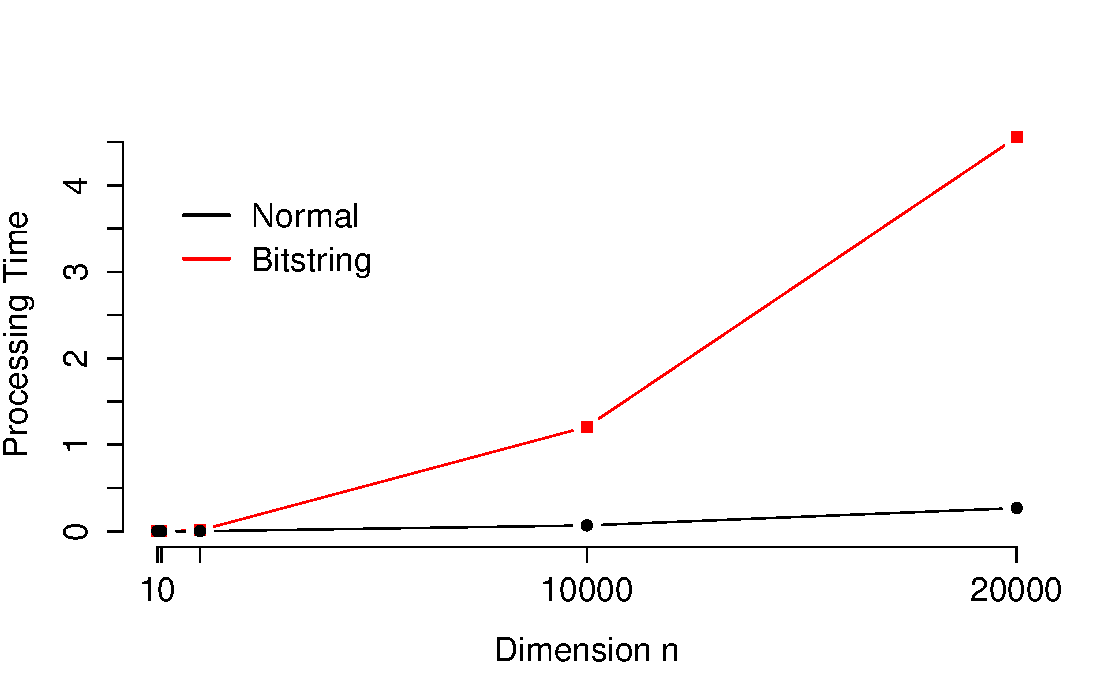
\includegraphics[scale=0.4,clip]{fig32}
  }
  \subfigure[$A=A+A$]{
   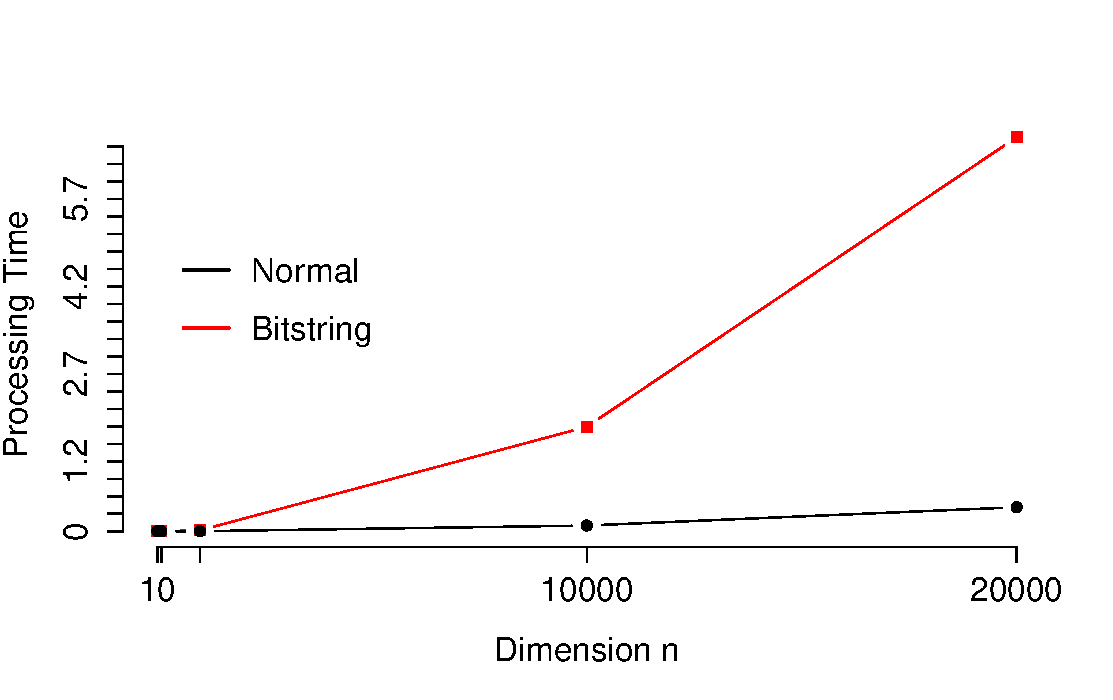
\includegraphics[scale=0.4,clip]{fig33}
  }
  \subfigure[$A=A-8.0000$]{
   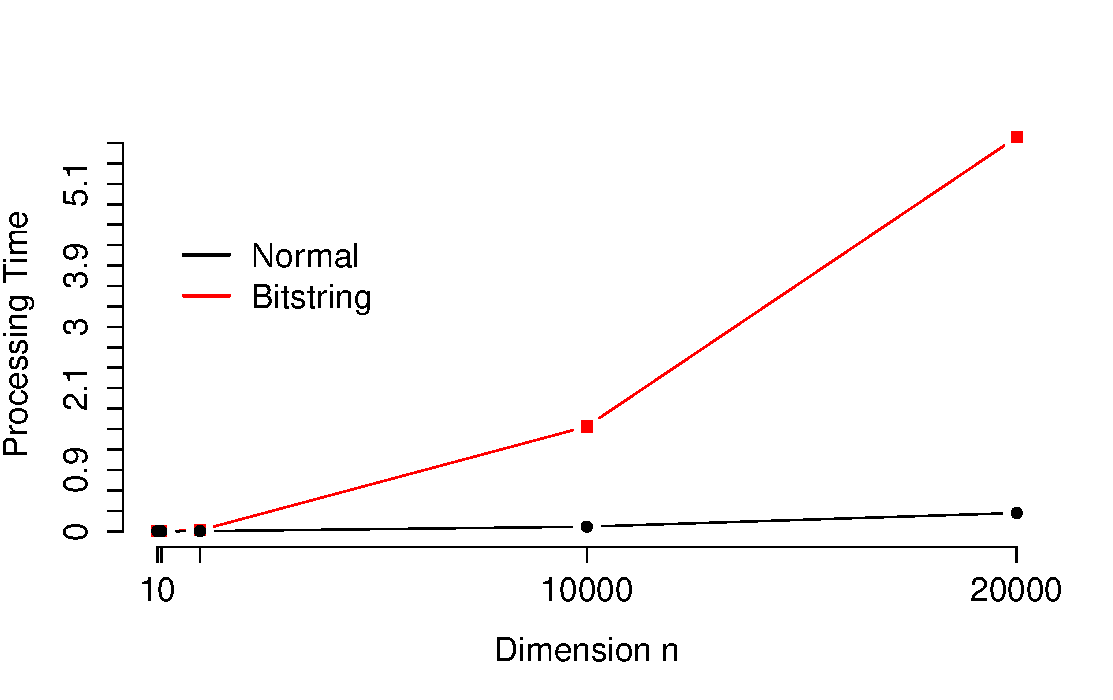
\includegraphics[scale=0.4,clip]{fig34}
  }
  \caption{Processing time of the following operations: attribution ($A=5.0000$, 
A is the matrix with an n by n dimension); 
  element sum of a matrix with a constant ($A=A+5.000$);sum of matrices 
($A=A+A$); and subtraction of the elements of a 
  matrix by a constant ($A=A-8.0000$) involving real numbers ($R$) and positive 
integer numbers ($R^+$). The bitstring 
  method presented the best overall performance only for the attribution 
operations, because the storage of 
  different numbers occurs in one element of a matrix, which reduces the 
accessing time. For the other operations, 
  the bitstring method is slower due to the number ofoperations which are 
necessary to be  executed in order to 
  access the elements. This can still be optimized in the implemented library.}
  \label{fig:31323334}
\end{figure}

\begin{figure}[h]
  \centering
  \subfigure[$A = A \times A$]{
   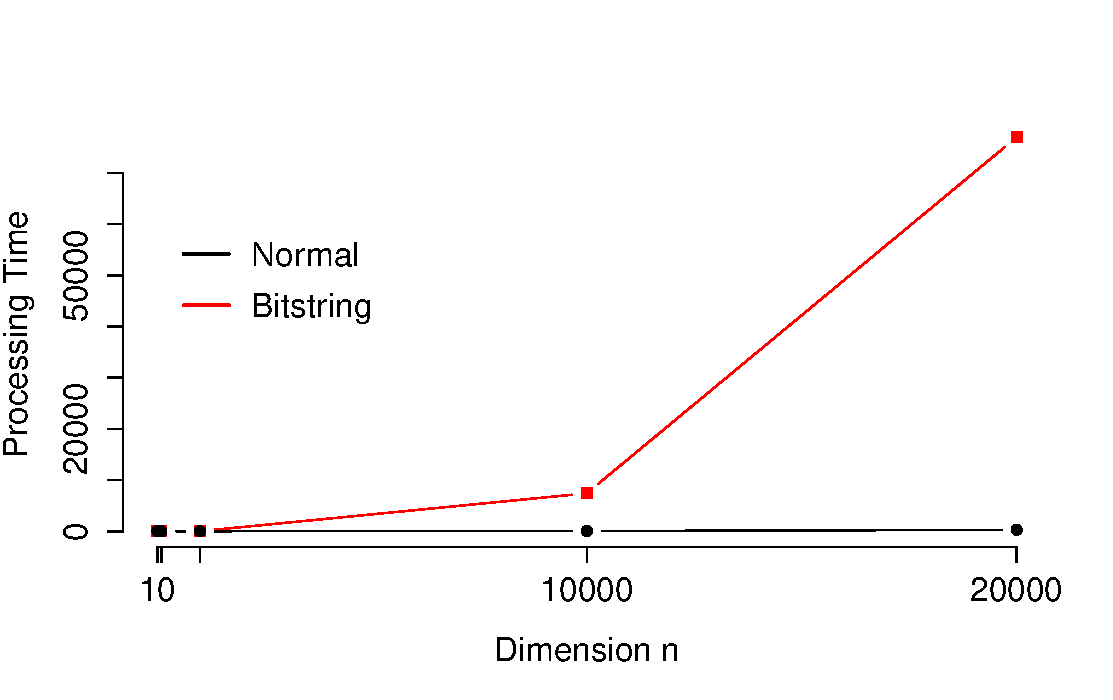
\includegraphics[scale=0.4,clip]{fig35}
  }
  \subfigure[$A=A \times 2$]{
   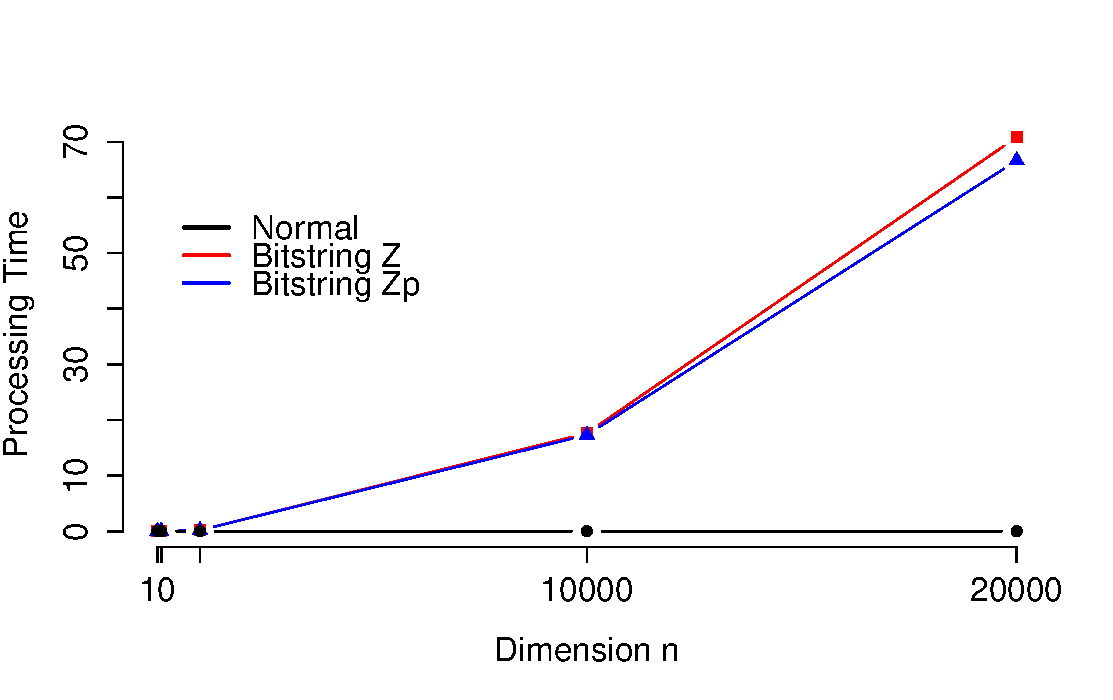
\includegraphics[scale=0.4,clip]{fig36}
  }
  \subfigure[$transpose(A)$]{
   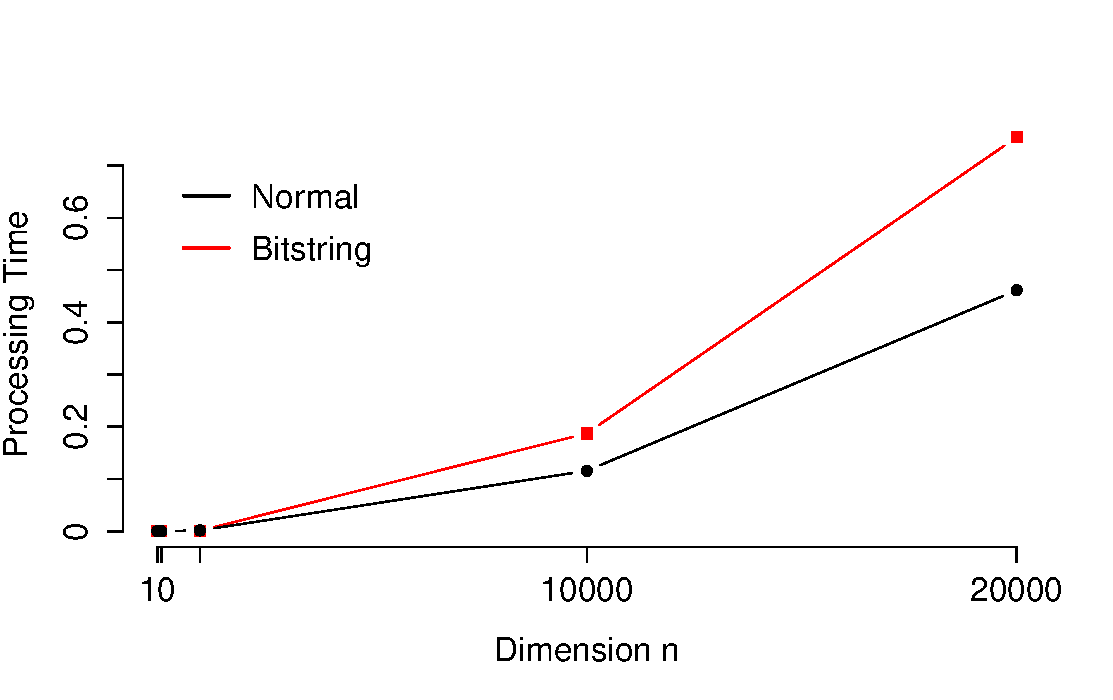
\includegraphics[scale=0.4,clip]{fig37}
  }
  \subfigure[$maximum(A)$]{
   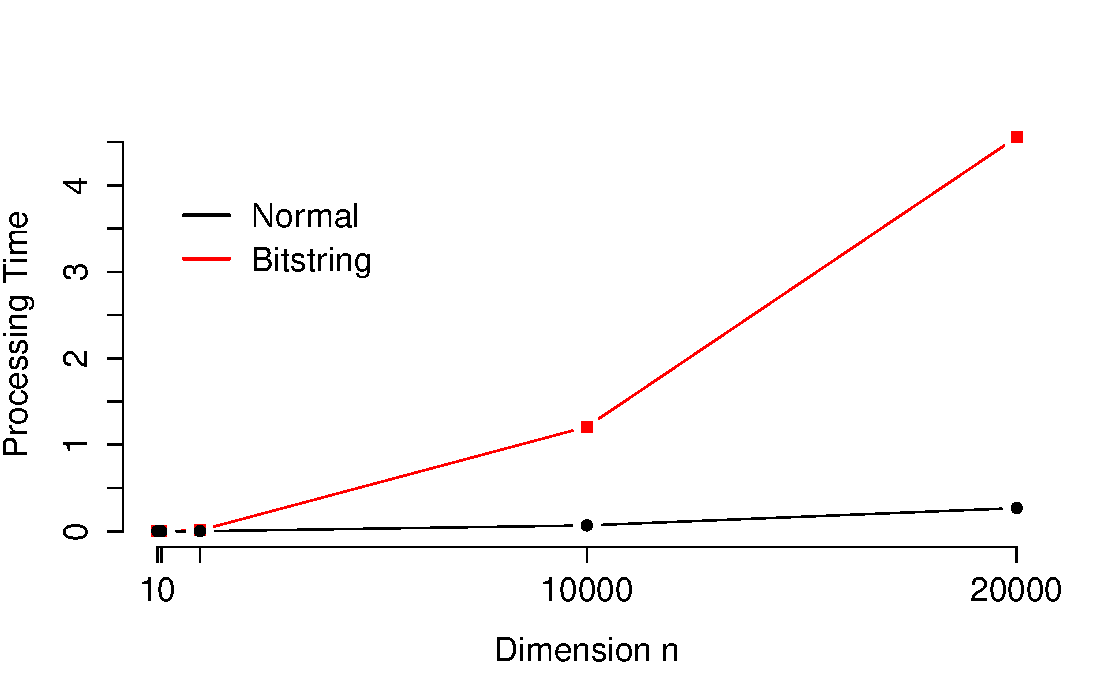
\includegraphics[scale=0.4,clip]{fig38}
  }
  \caption{Processing time of matrix multiplication ($A = A \times A$, A is the 
matrix with a n by n dimension), 
  element multiplication of matrix by constant ($A=A \times 2.0000$), the 
calculation of transpose and maximum of a 
  matrix involve integer numbers ($R$) and positive integer numbers ($R^+$). In 
this cases, the traditional 
  method was faster than the bitstring model.}
  \label{fig:35363738}
\end{figure}

\begin{figure}[h]
  \centering
  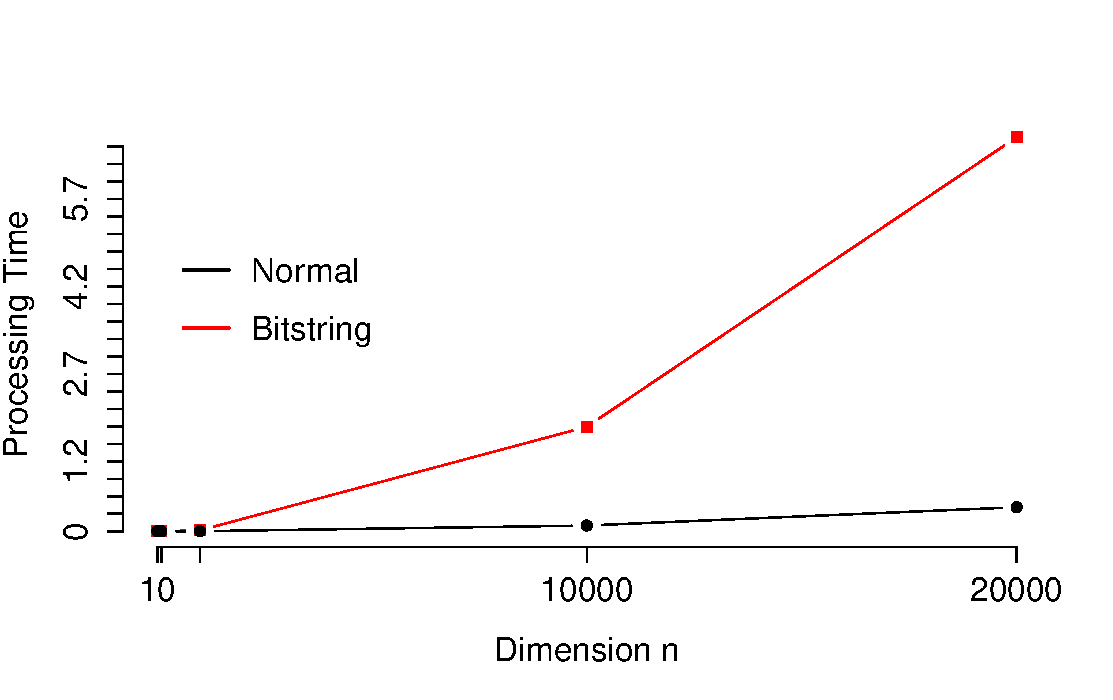
\includegraphics[scale=0.6,clip]{fig39}
  \caption{Processing time for the Per User Average method (PUA) in function of 
the numbers of linesof a matrix 
  with 3,000 columns. The vertical green line indicates the approximate moment 
when the traditional method  
  demands  disk access in order to store the matrix to be analyzed, which  
overloads the process. The bitstring 
  method fully represents a matrix  in memory, without the necessity to access 
the  disk.}
  \label{fig39}
\end{figure}

\begin{figure}[h]
  \centering
  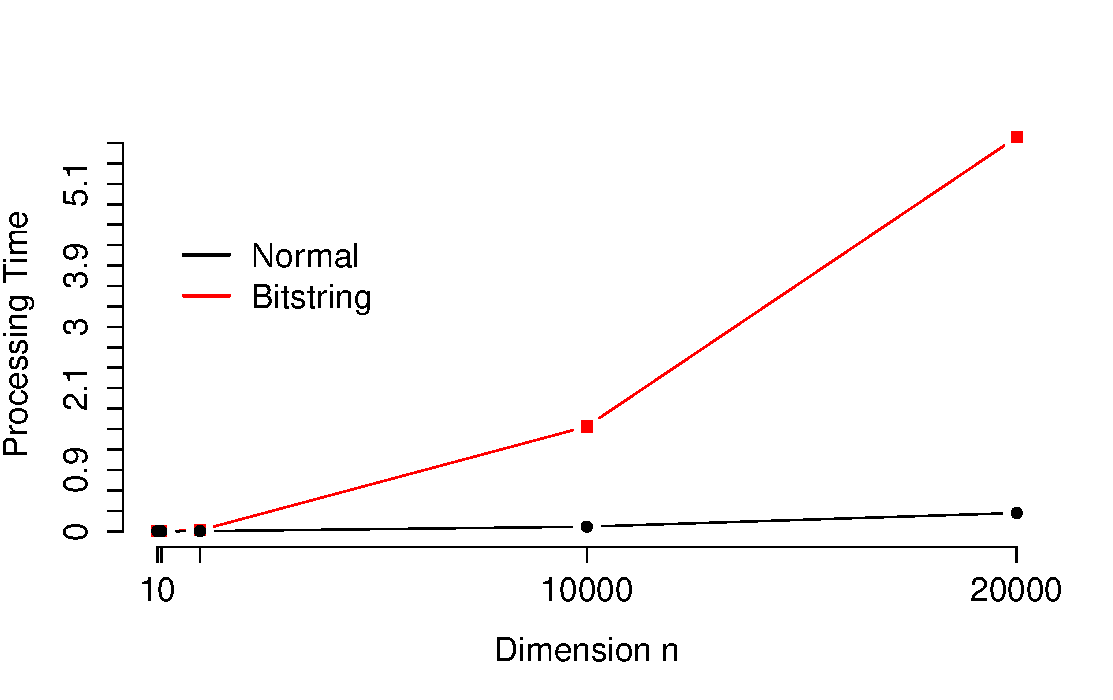
\includegraphics[scale=0.6,clip]{fig40}
  \caption{Processing time for the Per User Average method (PUA) in function of 
the  numbers of lines of a matrix 
  with 3,000 columns.  The vertical green line indicates the approximate moment 
when the traditional method  
  demands disk access in order to store the matrixto be analyzed, which  
overloads the process. For dimensions 
  inferior to approximately 400 lines, the traditional method is faster than the 
bitstring one. It is important 
  to emphasize that the computational cost of both methods is linear.}
  \label{fig40}
\end{figure}

\begin{figure}[h]
  \centering
  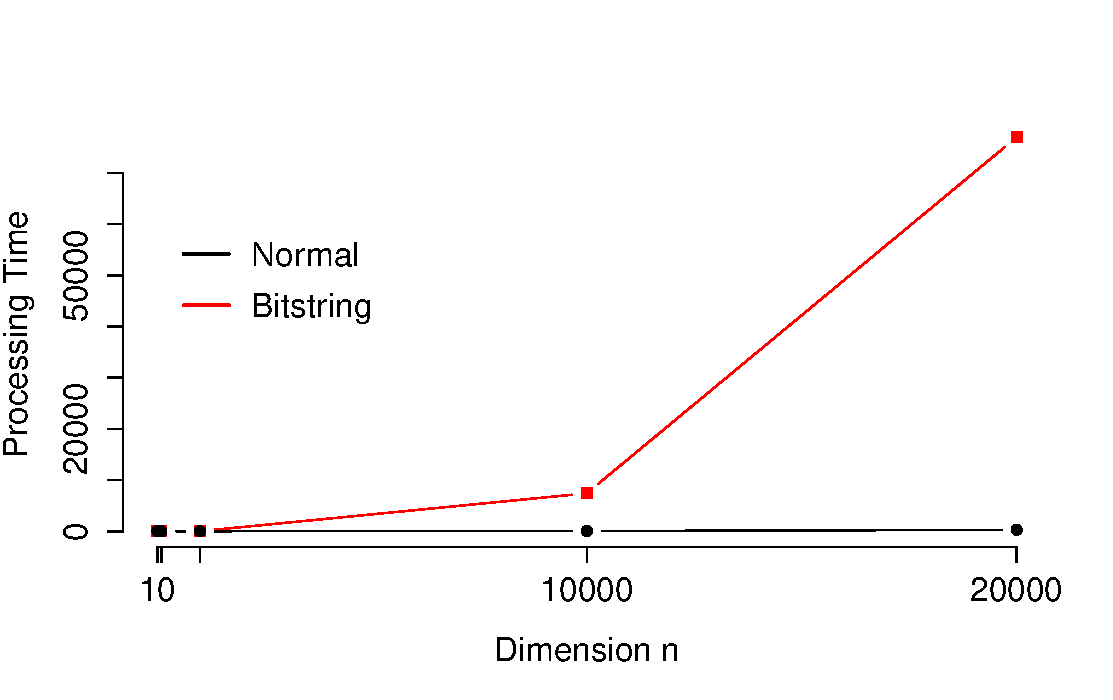
\includegraphics[scale=0.6,clip]{fig41}
  \caption{Relation between the processing time using the bitstring method and 
the traditional method in function 
  of the line numbers of a matrix with 3,000 columns. It is possible to verify 
that for a matrix with less than 400 
  lines, the traditional method is faster. However, when the number of lines is 
greater  than 400 lines, the best 
  method is the bitstring because of the compressed representation in the matrix 
memory.}
  \label{fig41}
\end{figure}

\begin{figure}[h]
  \centering
  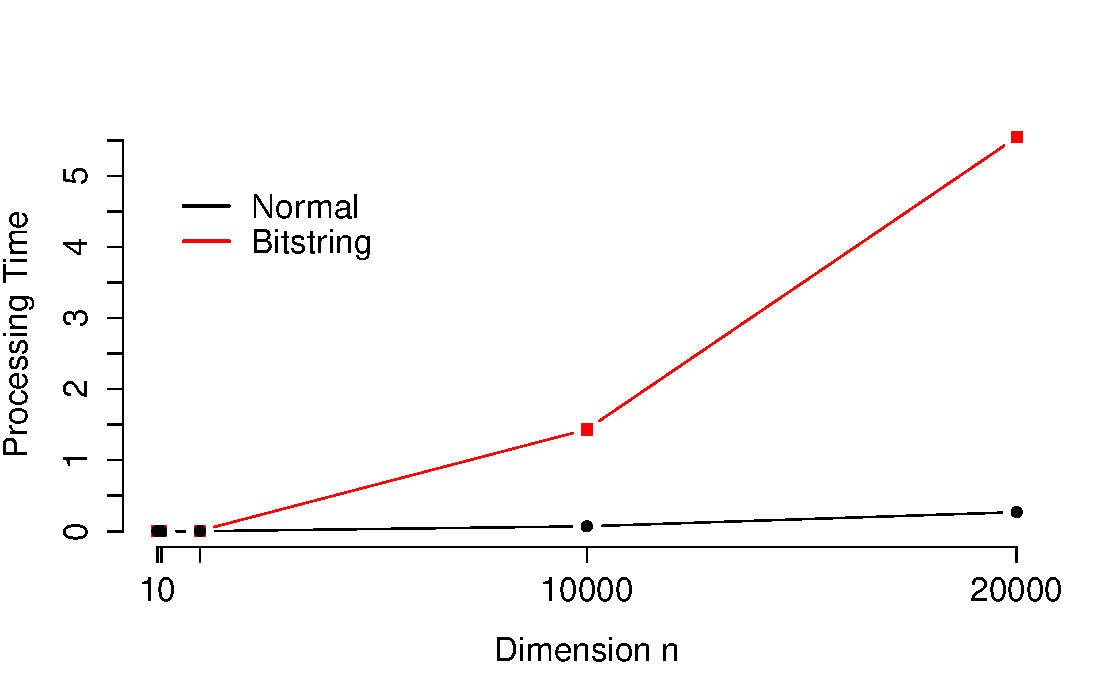
\includegraphics[scale=0.6,clip]{fig42}
  \caption{Processing time for the Bias From Mean method (BMF) in function of 
the numbers of linesof a matrix 
  with 3,000 columns. The vertical green line indicates the approximate moment 
when the traditional method  
  demands  disk access in order to store the matrix to be analyzed, which  
overloads the process. The bitstring 
  method fully represents a matrix  in memory, without the necessity to access 
the  disk.}
  \label{fig42}
\end{figure}

\begin{figure}[h]
  \centering
  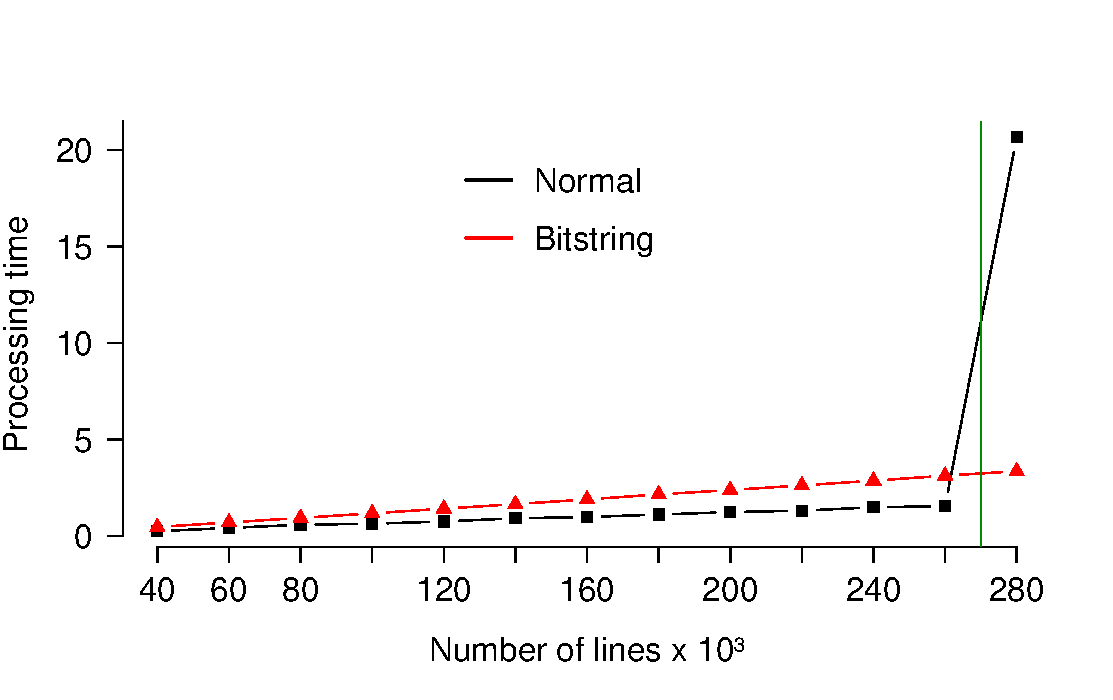
\includegraphics[scale=0.6,clip]{fig43}
  \caption{Processing time for the Bias From Mean method (BMF) in function of 
the  numbers of lines of a matrix 
  with 3,000 columns.  The vertical green line indicates the approximate moment 
when the traditional method  
  demands disk access in order to store the matrixto be analyzed, which  
overloads the process. For dimensions 
  inferior to approximately 400 lines, the traditional method is faster than the 
bitstring one. It is important 
  to emphasize that the computational cost of both methods is linear.}
  \label{fig43}
\end{figure}

\begin{figure}[h]
  \centering
  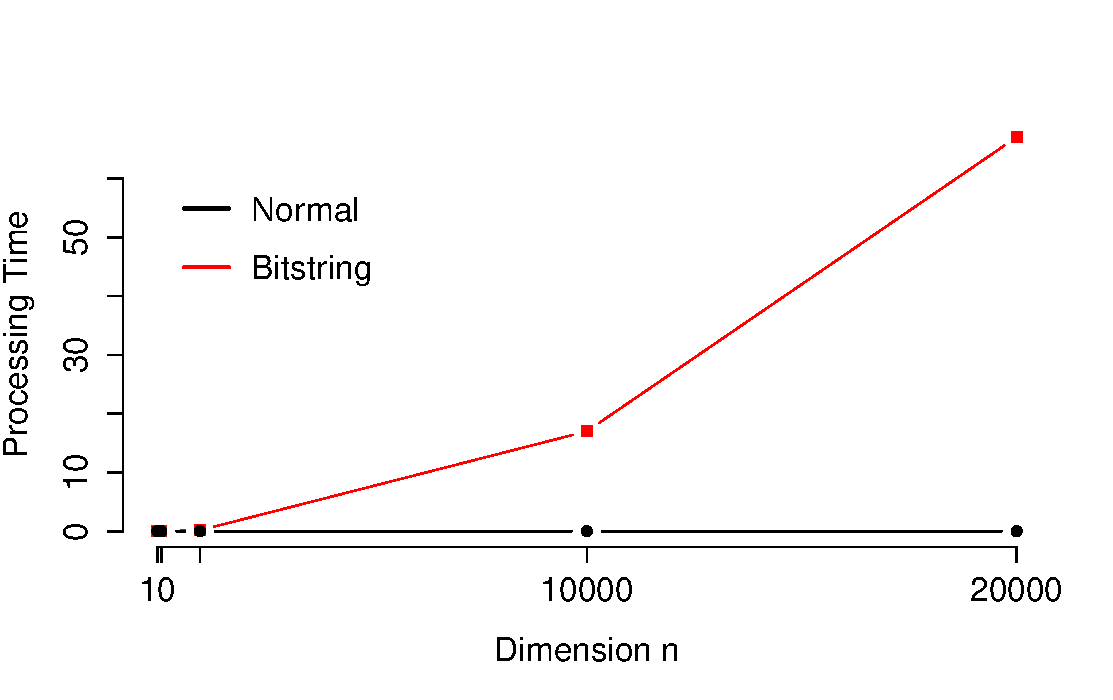
\includegraphics[scale=0.6,clip]{fig44}
  \caption{Relation between the processing time using the bitstring method and 
the traditional method in function 
  of the line numbers of a matrix with 3,000 columns. It is possible to verify 
that for a matrix with less than 400 
  lines, the traditional method is faster. However, when the number of lines is 
greater  than 400 lines, the best 
  method is the bitstring because of the compressed representation in the matrix 
memory.}
  \label{fig44}
\end{figure}



%\begin{figure}[!ht]
%\begin{center}
%%\includegraphics[width=4in]{figure_name.2.eps}
%\end{center}
%\caption{
%{\bf Bold the first sentence.}  Rest of figure 2  caption.  Caption 
%should be left justified, as specified by the options to the caption 
%package.
%}
%\label{Figure_label}
%\end{figure}

\newpage

\clearpage


\bibliography{plos.bib}
\end{document}
